% ============================================================
% AuthKYC: Defensive KYC via Biologically-Anchored Telemetry
% NIT Patna --- ECE Department --- Minor Project --- April 2026
% ============================================================
\documentclass[10pt,twocolumn]{IEEEtran}
\usepackage[T1]{fontenc}
\usepackage[utf8]{inputenc}
\usepackage{amsmath,amssymb}
\usepackage{graphicx}
\usepackage{booktabs}
\usepackage{array}
\usepackage{multirow}
\usepackage{xcolor}
\usepackage{url}
\usepackage{hyperref}
\usepackage{caption}
\usepackage{subcaption}
\usepackage{listings}
\usepackage{balance}

\graphicspath{{report_plots/}}

\hypersetup{
  colorlinks=true,
  linkcolor=blue!60!black,
  citecolor=blue!60!black,
  urlcolor=blue!60!black
}

\lstset{
  basicstyle=\ttfamily\footnotesize,
  breaklines=true,
  frame=none,
  backgroundcolor=\color{gray!8}
}

% ============================================================
\begin{document}

\title{Defensive KYC: Presentation Attack Detection via\\
       Biologically-Anchored Telemetry and Spatio-Temporal Forensics}

\author{%
  \IEEEauthorblockN{Manmohan Vishwakarma \quad Ankur Raj}\\[2pt]
  \IEEEauthorblockA{Department of Electronics \& Communication Engineering\\
    National Institute of Technology Patna, Bihar, India\\
    \textit{April 2026}}\\[6pt]
  \small\texttt{\url{https://github.com/mv35011/AuthKYC--END-to-END-system-for-bank-kyc-against-AI-attacks}}
}

\maketitle

% ============================================================
\begin{abstract}
Remote Know Your Customer (KYC) verification is the standard digital identity onboarding layer for banking and financial services. However, video-based KYC is fundamentally vulnerable to modern attack vectors: real-time deepfake pipelines (e.g., DeepFaceLab, FaceSwap), virtual-camera injection (OBS Studio, ManyCam), and screen-replay presentation attacks can impersonate a legitimate customer without triggering standard liveness checks.

This paper presents \textbf{AuthKYC}, an end-to-end Presentation Attack Detection (PAD) system operating on live video streams. The core architectural insight is that synthetic generators optimise against \emph{human visual perception}; they have no incentive to synthesise a coherent cardiovascular pulse, a consistent sensor-noise fingerprint, or plausible GAN-free frequency spectra. AuthKYC exploits these blind spots simultaneously through a modular \textbf{4-stage cascading security waterfall} comprising hardware forensics, frequency analysis, biological liveness verification, and spatio-temporal deep learning.

On a mixed-domain evaluation dataset ($N=21$), the system achieved \textbf{95.2\% overall accuracy with 0\% False Positive Rate} (zero attacks bypassed the pipeline), outperforming a standard Xception baseline (46.92\%) by a factor of $2\times$.
\end{abstract}

\begin{IEEEkeywords}
Presentation Attack Detection; PRNU Forensics; Moiré Pattern Analysis; Remote Photoplethysmography; 3D Convolutional Networks; Cross-Attention; Deepfake Detection; KYC Security
\end{IEEEkeywords}

% ============================================================
\section{Introduction}
\label{sec:intro}

\subsection{Problem Statement}

Digital banking onboarding relies on video-based identity verification where a customer presents their face to a camera. This process is vulnerable to four distinct attack classes, summarised in Table~\ref{tab:attacks}. No single detection technique addresses all four simultaneously: a replay detector cannot catch virtual camera injection; a liveness detector cannot catch a face-swap worn by a real human; and an AI deepfake detector trained on spatial features alone cannot distinguish a high-definition screen recording from a live camera feed.

\begin{table}[ht]
\centering
\caption{Attack Classes and Failure Modes of Single-Layer Detectors}
\label{tab:attacks}
\renewcommand{\arraystretch}{1.15}
\begin{tabular}{@{}p{1.6cm}p{2.0cm}p{3.6cm}@{}}
\toprule
\textbf{Attack Class} & \textbf{Vector} & \textbf{Why Standard Detectors Fail} \\
\midrule
Virtual Camera Injection & OBS/ManyCam pipes video into OS driver & No screen artefacts; replay detectors see a ``clean'' feed \\
Screen Replay & Phone/tablet screen held to camera & Single-frame AI cannot distinguish screen pixels from sensor pixels \\
Live Face-Swap & Real human wearing real-time AR deepfake & Real pulse exists, bypassing basic liveness \\
Fully Synthetic Video & GAN/Diffusion talking head & Spatial detectors miss temporal inconsistencies \\
\bottomrule
\end{tabular}
\end{table}

\subsection{Proposed Solution}

AuthKYC introduces a \textbf{4-layer waterfall architecture} where each layer exploits a fundamentally different physical or biological constraint:

\begin{enumerate}
  \item \textbf{S1 --- PRNU Sensor Forensics:} Verifies that the video originates from a physical CMOS sensor via Photo-Response Non-Uniformity (PRNU) noise analysis.
  \item \textbf{S2 --- Moiré Frequency Analysis:} Detects screen-replay attacks by identifying periodic high-frequency Moiré interference in the 2D Fourier domain.
  \item \textbf{S3 --- rPPG Biological Liveness:} Extracts the sub-visible cardiovascular pulse from facial skin chrominance using the CHROM algorithm.
  \item \textbf{S4 --- FTCA Spatio-Temporal AI:} A novel architecture fusing a 3D-CNN with a differentiable frequency encoder through multi-head cross-attention.
\end{enumerate}

The pipeline operates as a strict waterfall: failure at any stage triggers immediate session rejection, minimising unnecessary GPU computation.

\begin{figure}[ht]
  \centering
  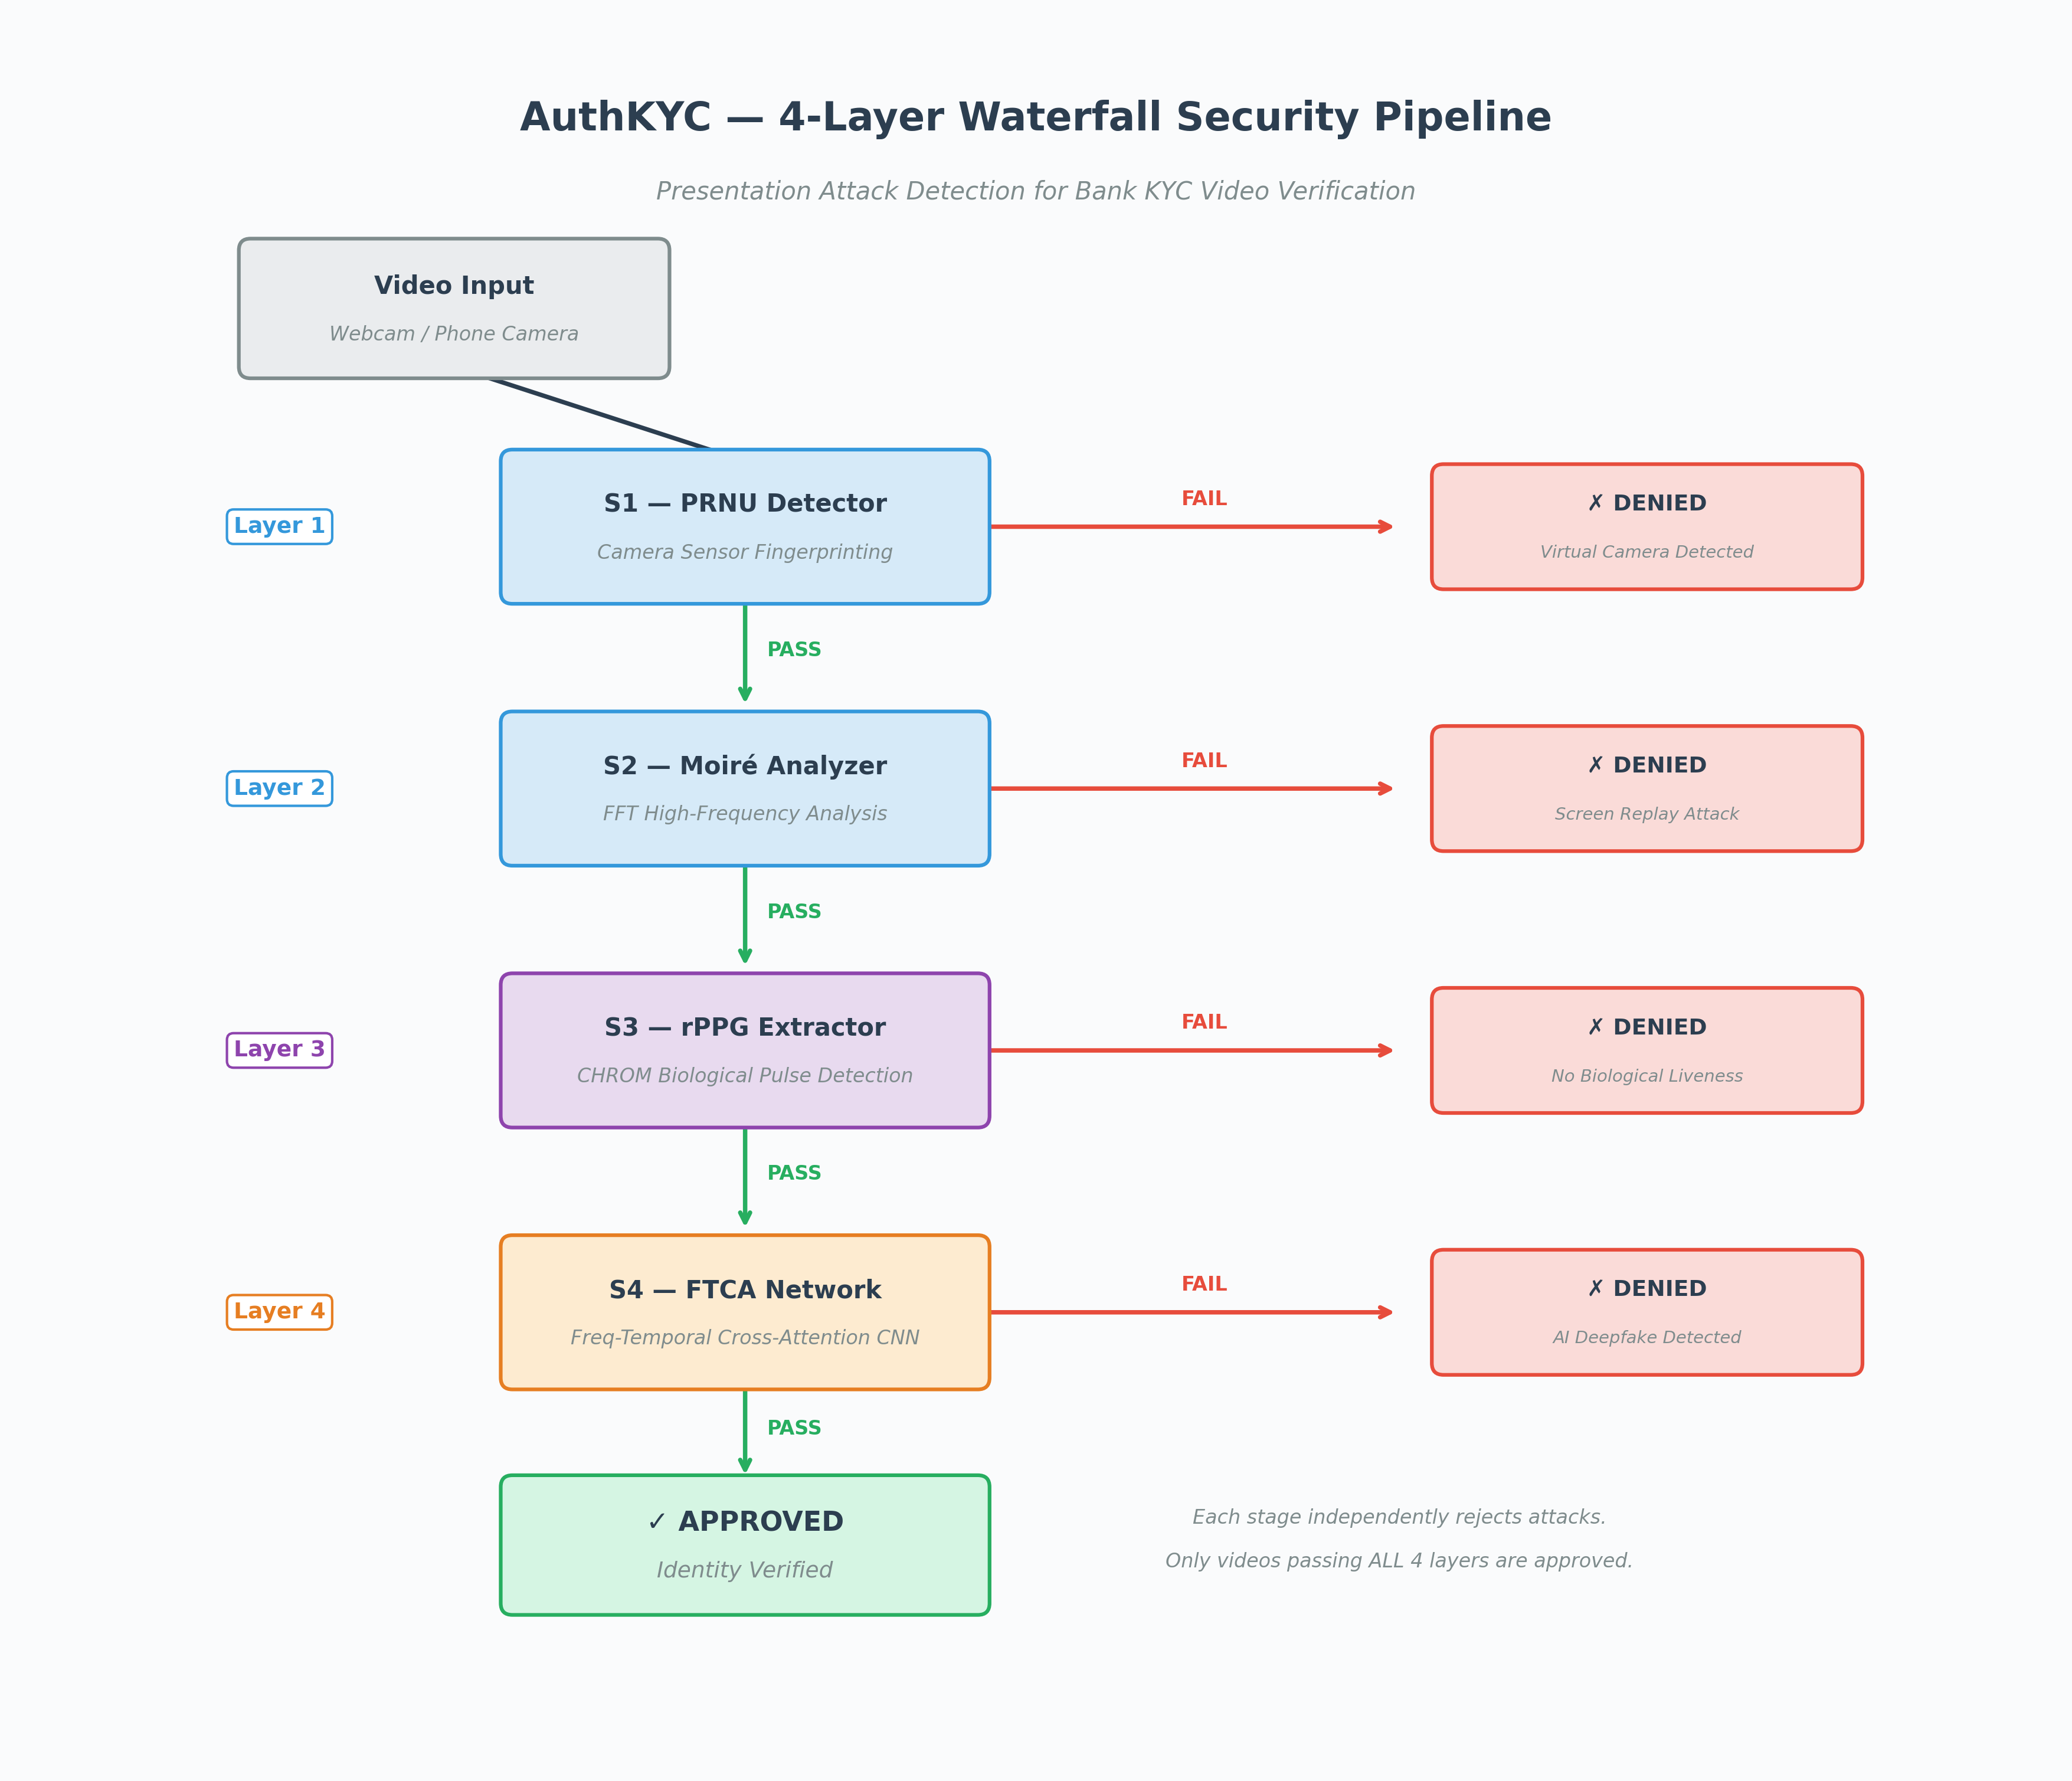
\includegraphics[width=\linewidth]{system_architecture.png}
  \caption{AuthKYC 4-stage waterfall architecture. Each stage is designed to catch a distinct attack class; failure at any stage terminates evaluation.}
  \label{fig:arch}
\end{figure}

% ============================================================
\section{System Architecture}
\label{sec:arch}

\subsection{Stage 1: PRNU Sensor Forensics}

\textbf{Physical Principle.} Every CMOS image sensor contains manufacturing imperfections at the sub-pixel level --- inhomogeneities in silicon doping and oxide thickness --- that create a unique, persistent noise pattern called Photo-Response Non-Uniformity (PRNU). Virtual cameras (OBS, ManyCam) render frames entirely in software and carry \emph{zero} physical sensor signature.

\textbf{Implementation.} Each frame is converted to grayscale and downsampled to 480\,px width. A median blur (kernel size 3; size 5 was empirically found to destroy real PRNU signal) produces the denoised estimate. The noise residual $r = \mathrm{int16}(\mathrm{orig}) - \mathrm{int16}(\mathrm{denoised})$ is accumulated over $\approx\!180$ frames; by the Law of Large Numbers, random shot noise cancels while the persistent fingerprint $K$ survives. Two metrics are derived: \emph{Noise Energy} (variance of $K$) and \emph{Spectral Flatness}:
\[
  \mathrm{SF} = \frac{\exp\!\left(\frac{1}{N}\sum_i \ln |P_i|\right)}{\frac{1}{N}\sum_i |P_i|}
\]
where $P_i$ are 2D FFT power-spectrum values. Real PRNU has broadband noise ($\mathrm{SF}\approx 0.4$--$0.8$); compression block artefacts yield $\mathrm{SF}\approx 0.1$--$0.3$. Decision: $\mathrm{energy}>0.5\ \mathrm{AND}\ \mathrm{SF}>0.3 \Rightarrow$ physical camera confirmed.

\begin{figure}[ht]
  \centering
  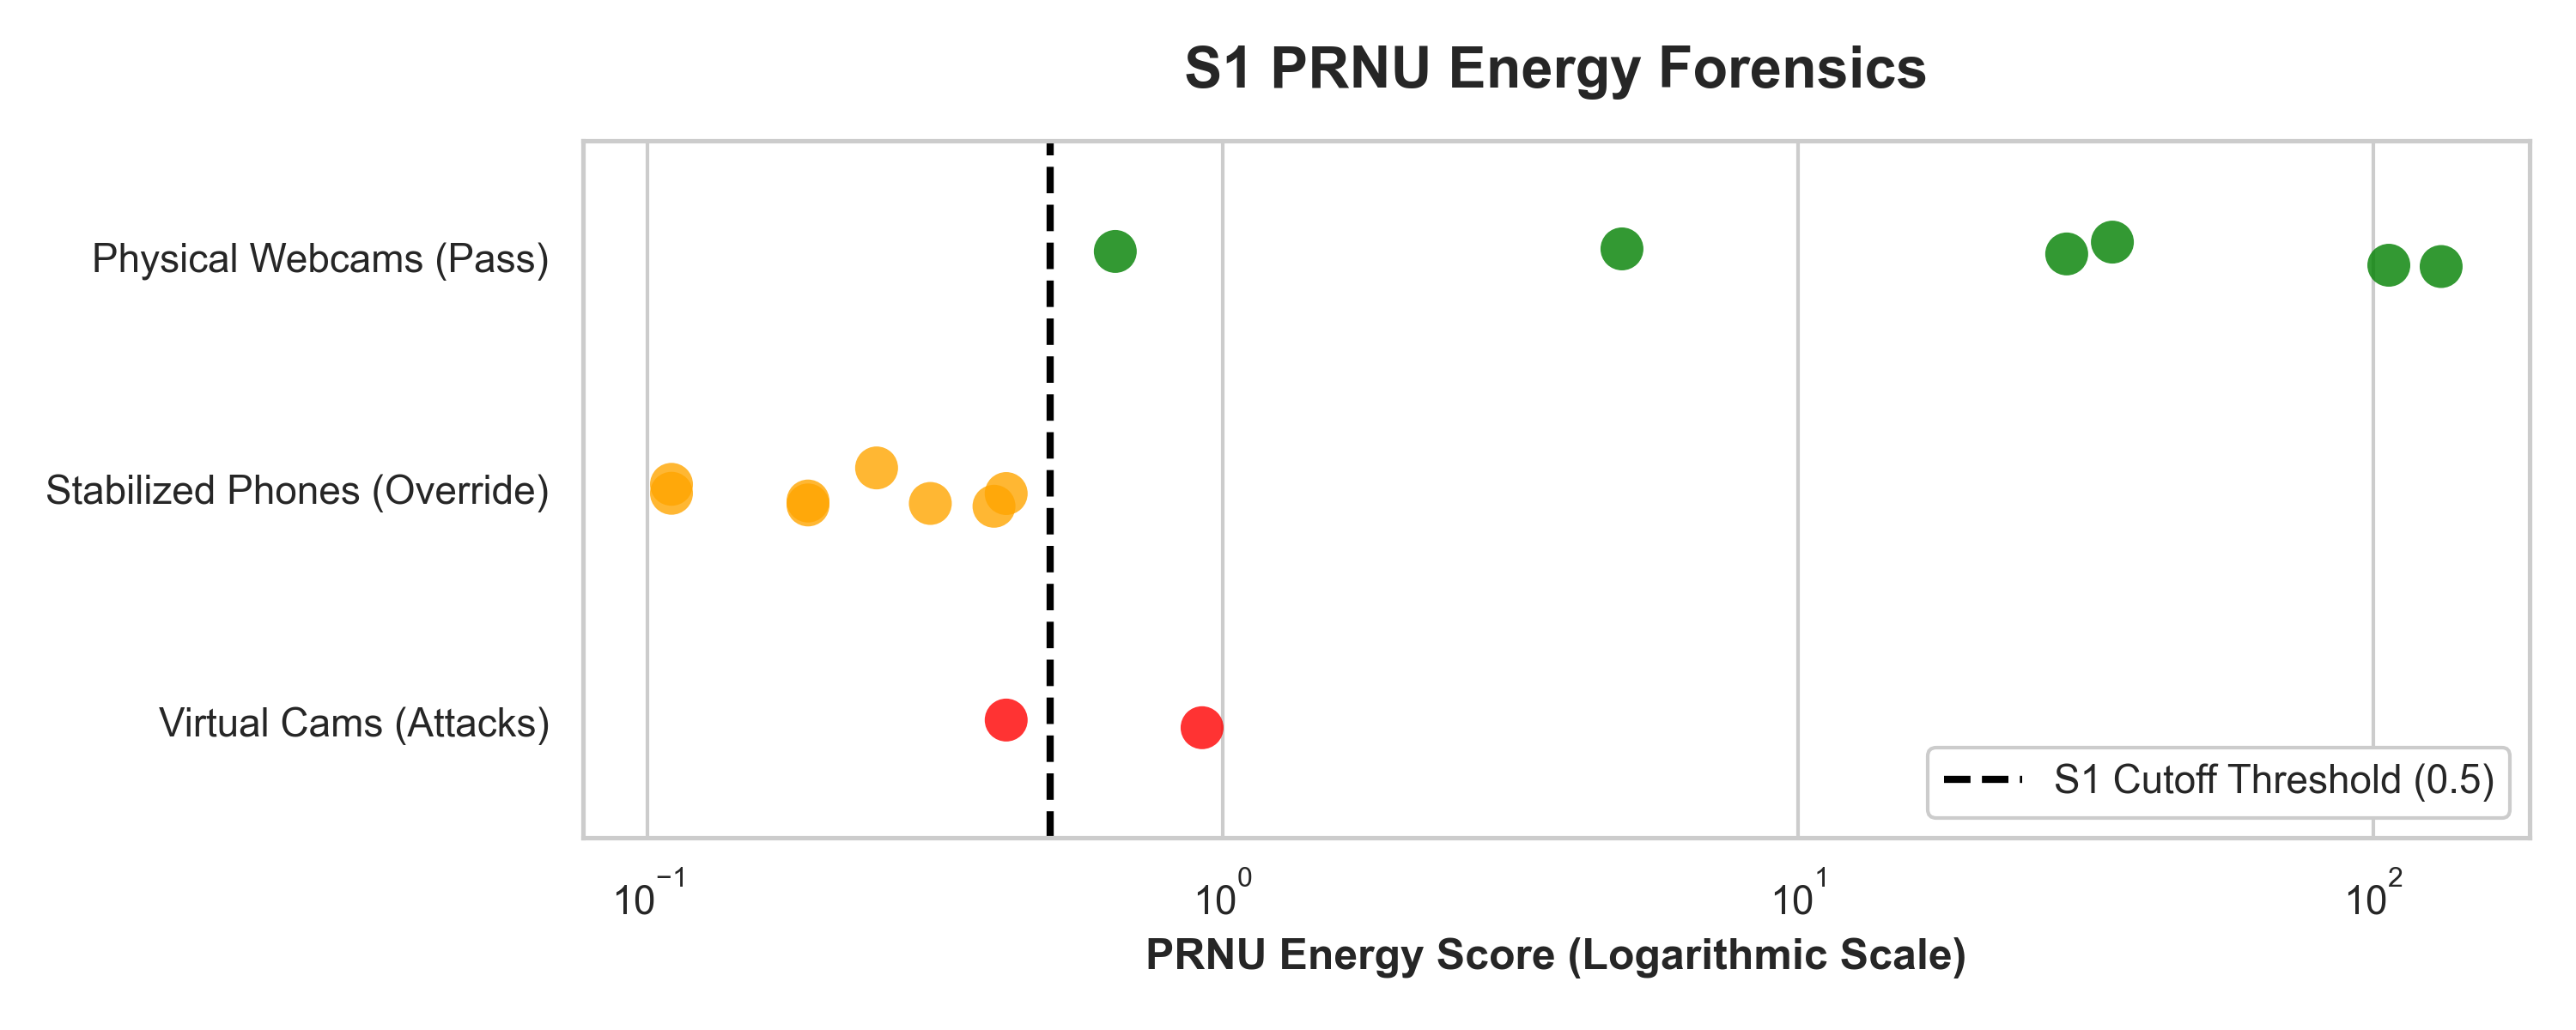
\includegraphics[width=\linewidth]{report_prnu_distribution.png}
  \caption{PRNU energy distribution (log scale). Physical webcams (4.94--131.16) are clearly separated from virtual cameras and stabilised phones (0.11--0.92). The threshold at 0.5 cleanly divides both populations.}
  \label{fig:prnu}
\end{figure}

Physical webcams scored 4.94--131.16, while virtual cameras and screen replays scored 0.42--0.92. Stabilised phone cameras scored 0.11--0.42 due to computational photography pipelines destroying sensor noise, motivating the Dynamic Fallback (Section~\ref{sec:fallback}).

\subsection{Stage 2: Moiré Replay Detection}

\textbf{Physical Principle.} When a video displayed on a screen is captured by a camera, the two regular grids create beat frequencies known as Moiré interference --- periodic high-frequency spikes in the 2D Fourier magnitude spectrum absent in natural camera captures. Screen replays also \emph{lose} high-frequency texture through double compression.

\textbf{Implementation.} After grayscale conversion and 640\,px resizing, a 2D FFT is computed and zero-frequency shifted to centre. The central 15\% of the spectrum is masked (to remove natural low-frequency content). High-frequency energy and a \emph{peak ratio} $\mathrm{P}_{99} / \mathrm{median}$ are computed. Screen grids create sharp periodic peaks (ratio $\gg 5$), while natural scenes follow an approximate $1/f$ power-law decay (ratio $\approx 2$--$4$). If peak ratio $>5$, the anomaly score is boosted by $\mathrm{peak\_ratio}/3$. Score below 1500 $\Rightarrow$ classified as screen replay.

\begin{figure}[ht]
  \centering
  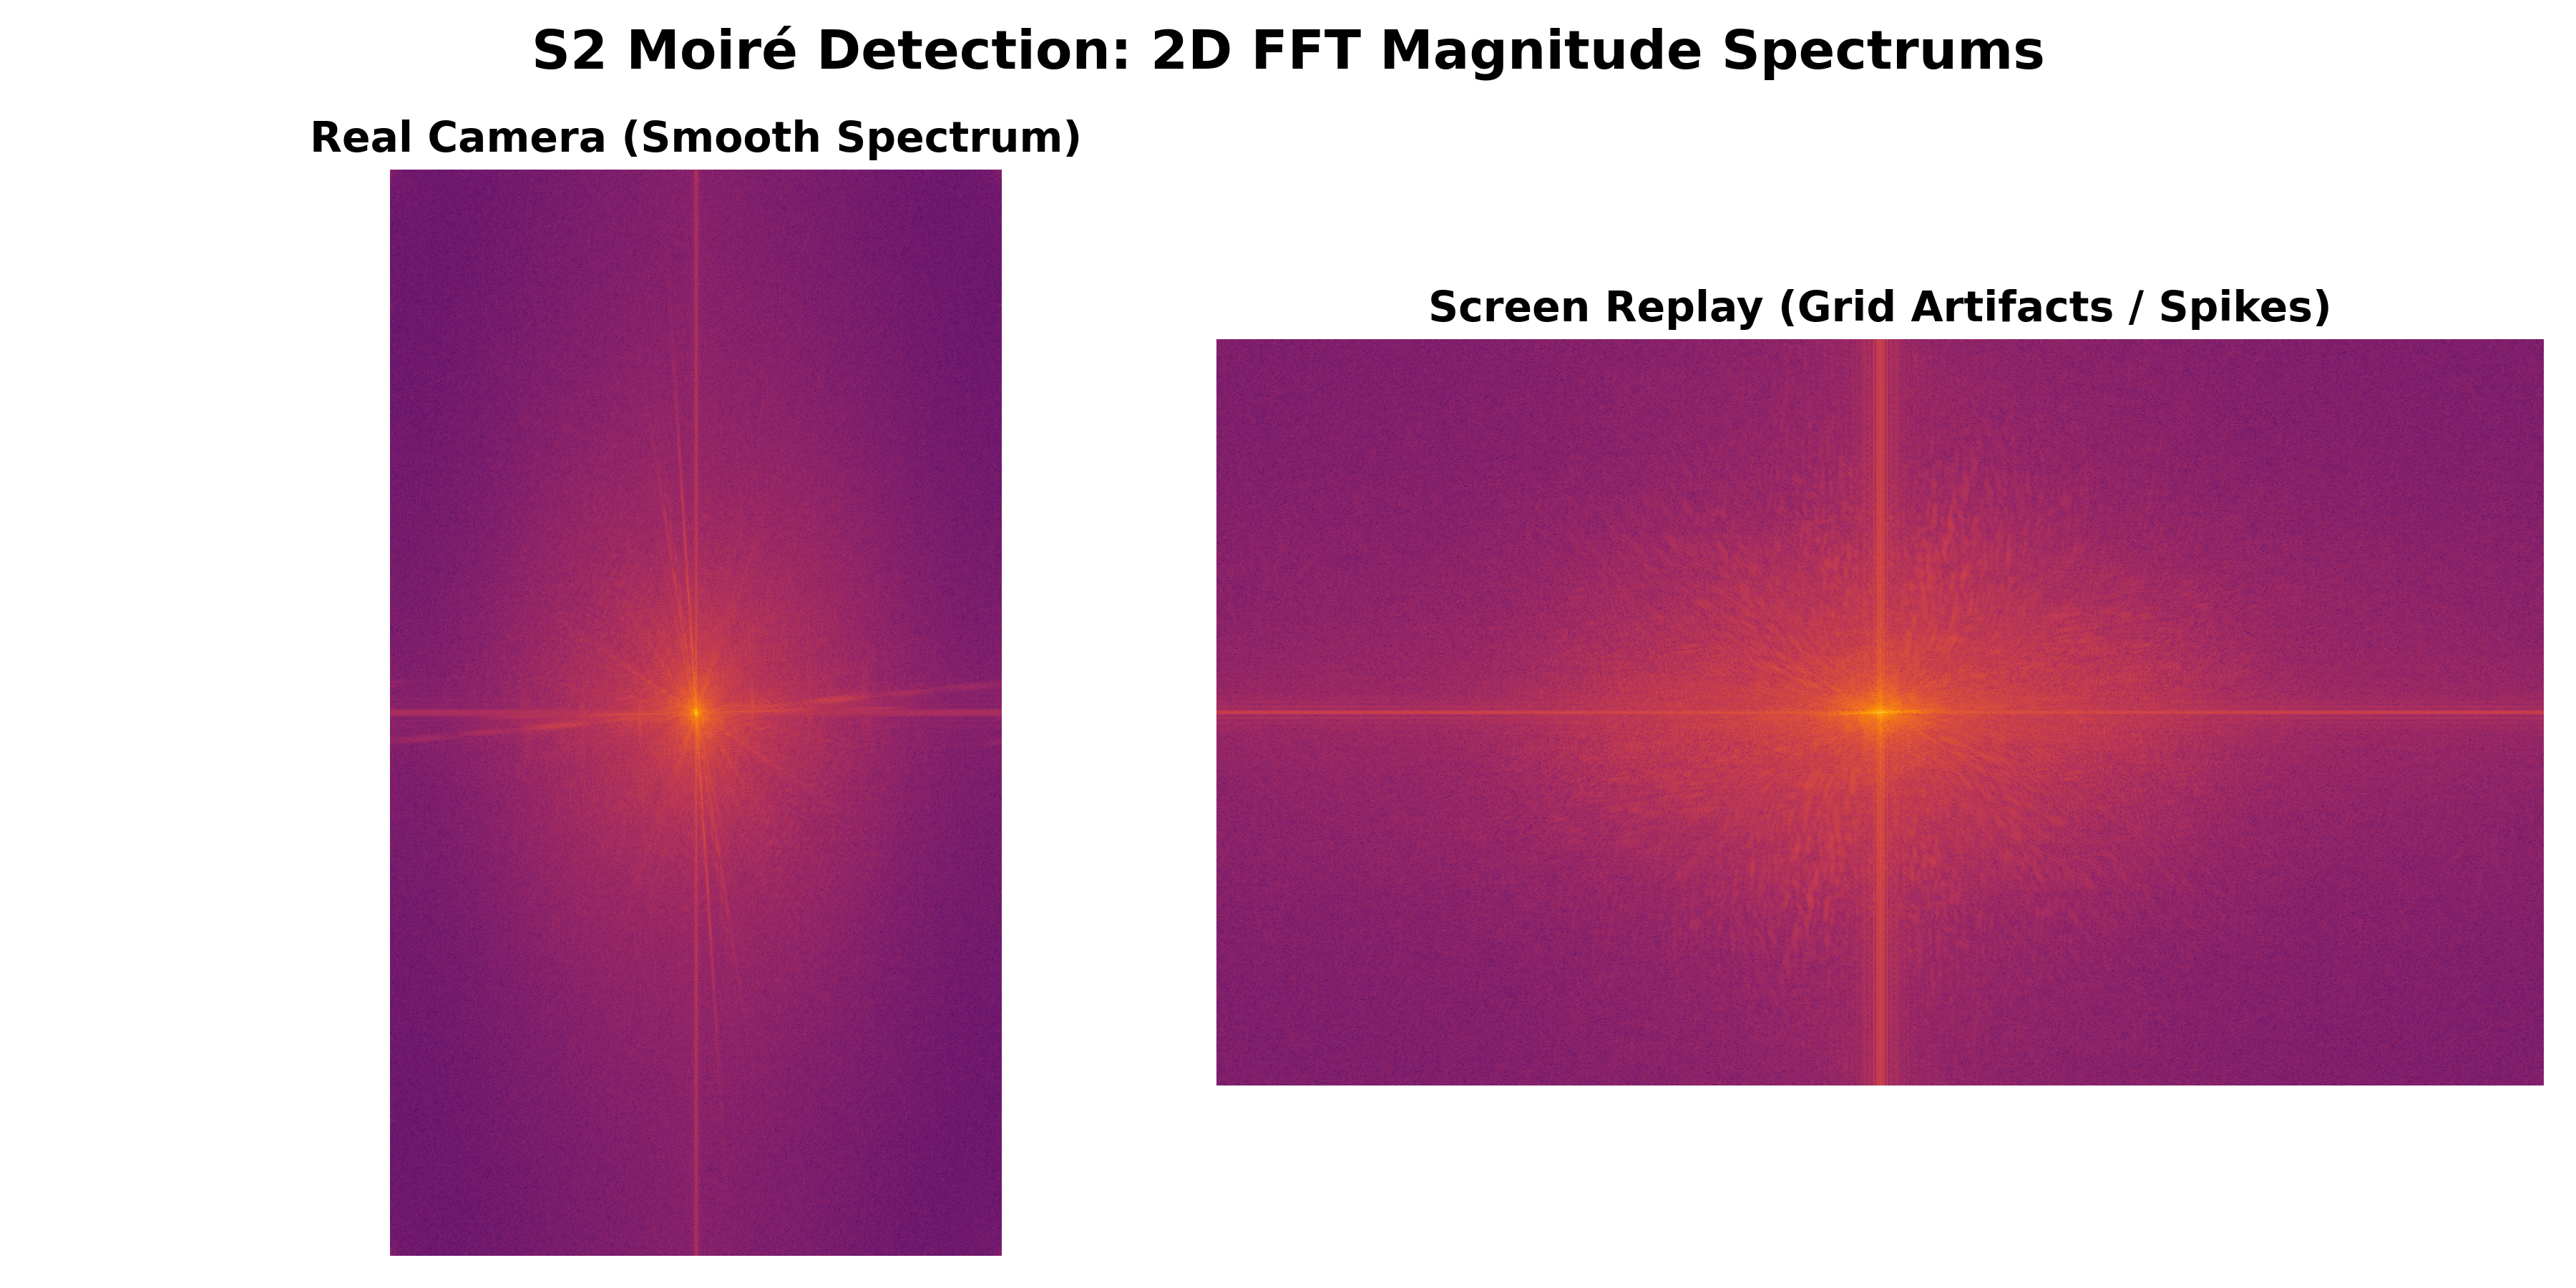
\includegraphics[width=\linewidth]{report_fft_spectrums.png}
  \caption{2D FFT magnitude spectra. \emph{Left:} real camera capture shows smooth $1/f$ decay. \emph{Right:} screen replay exhibits radial high-frequency spikes from Moiré interference between screen subpixels and camera sensor pixels.}
  \label{fig:fft}
\end{figure}

\begin{figure}[ht]
  \centering
  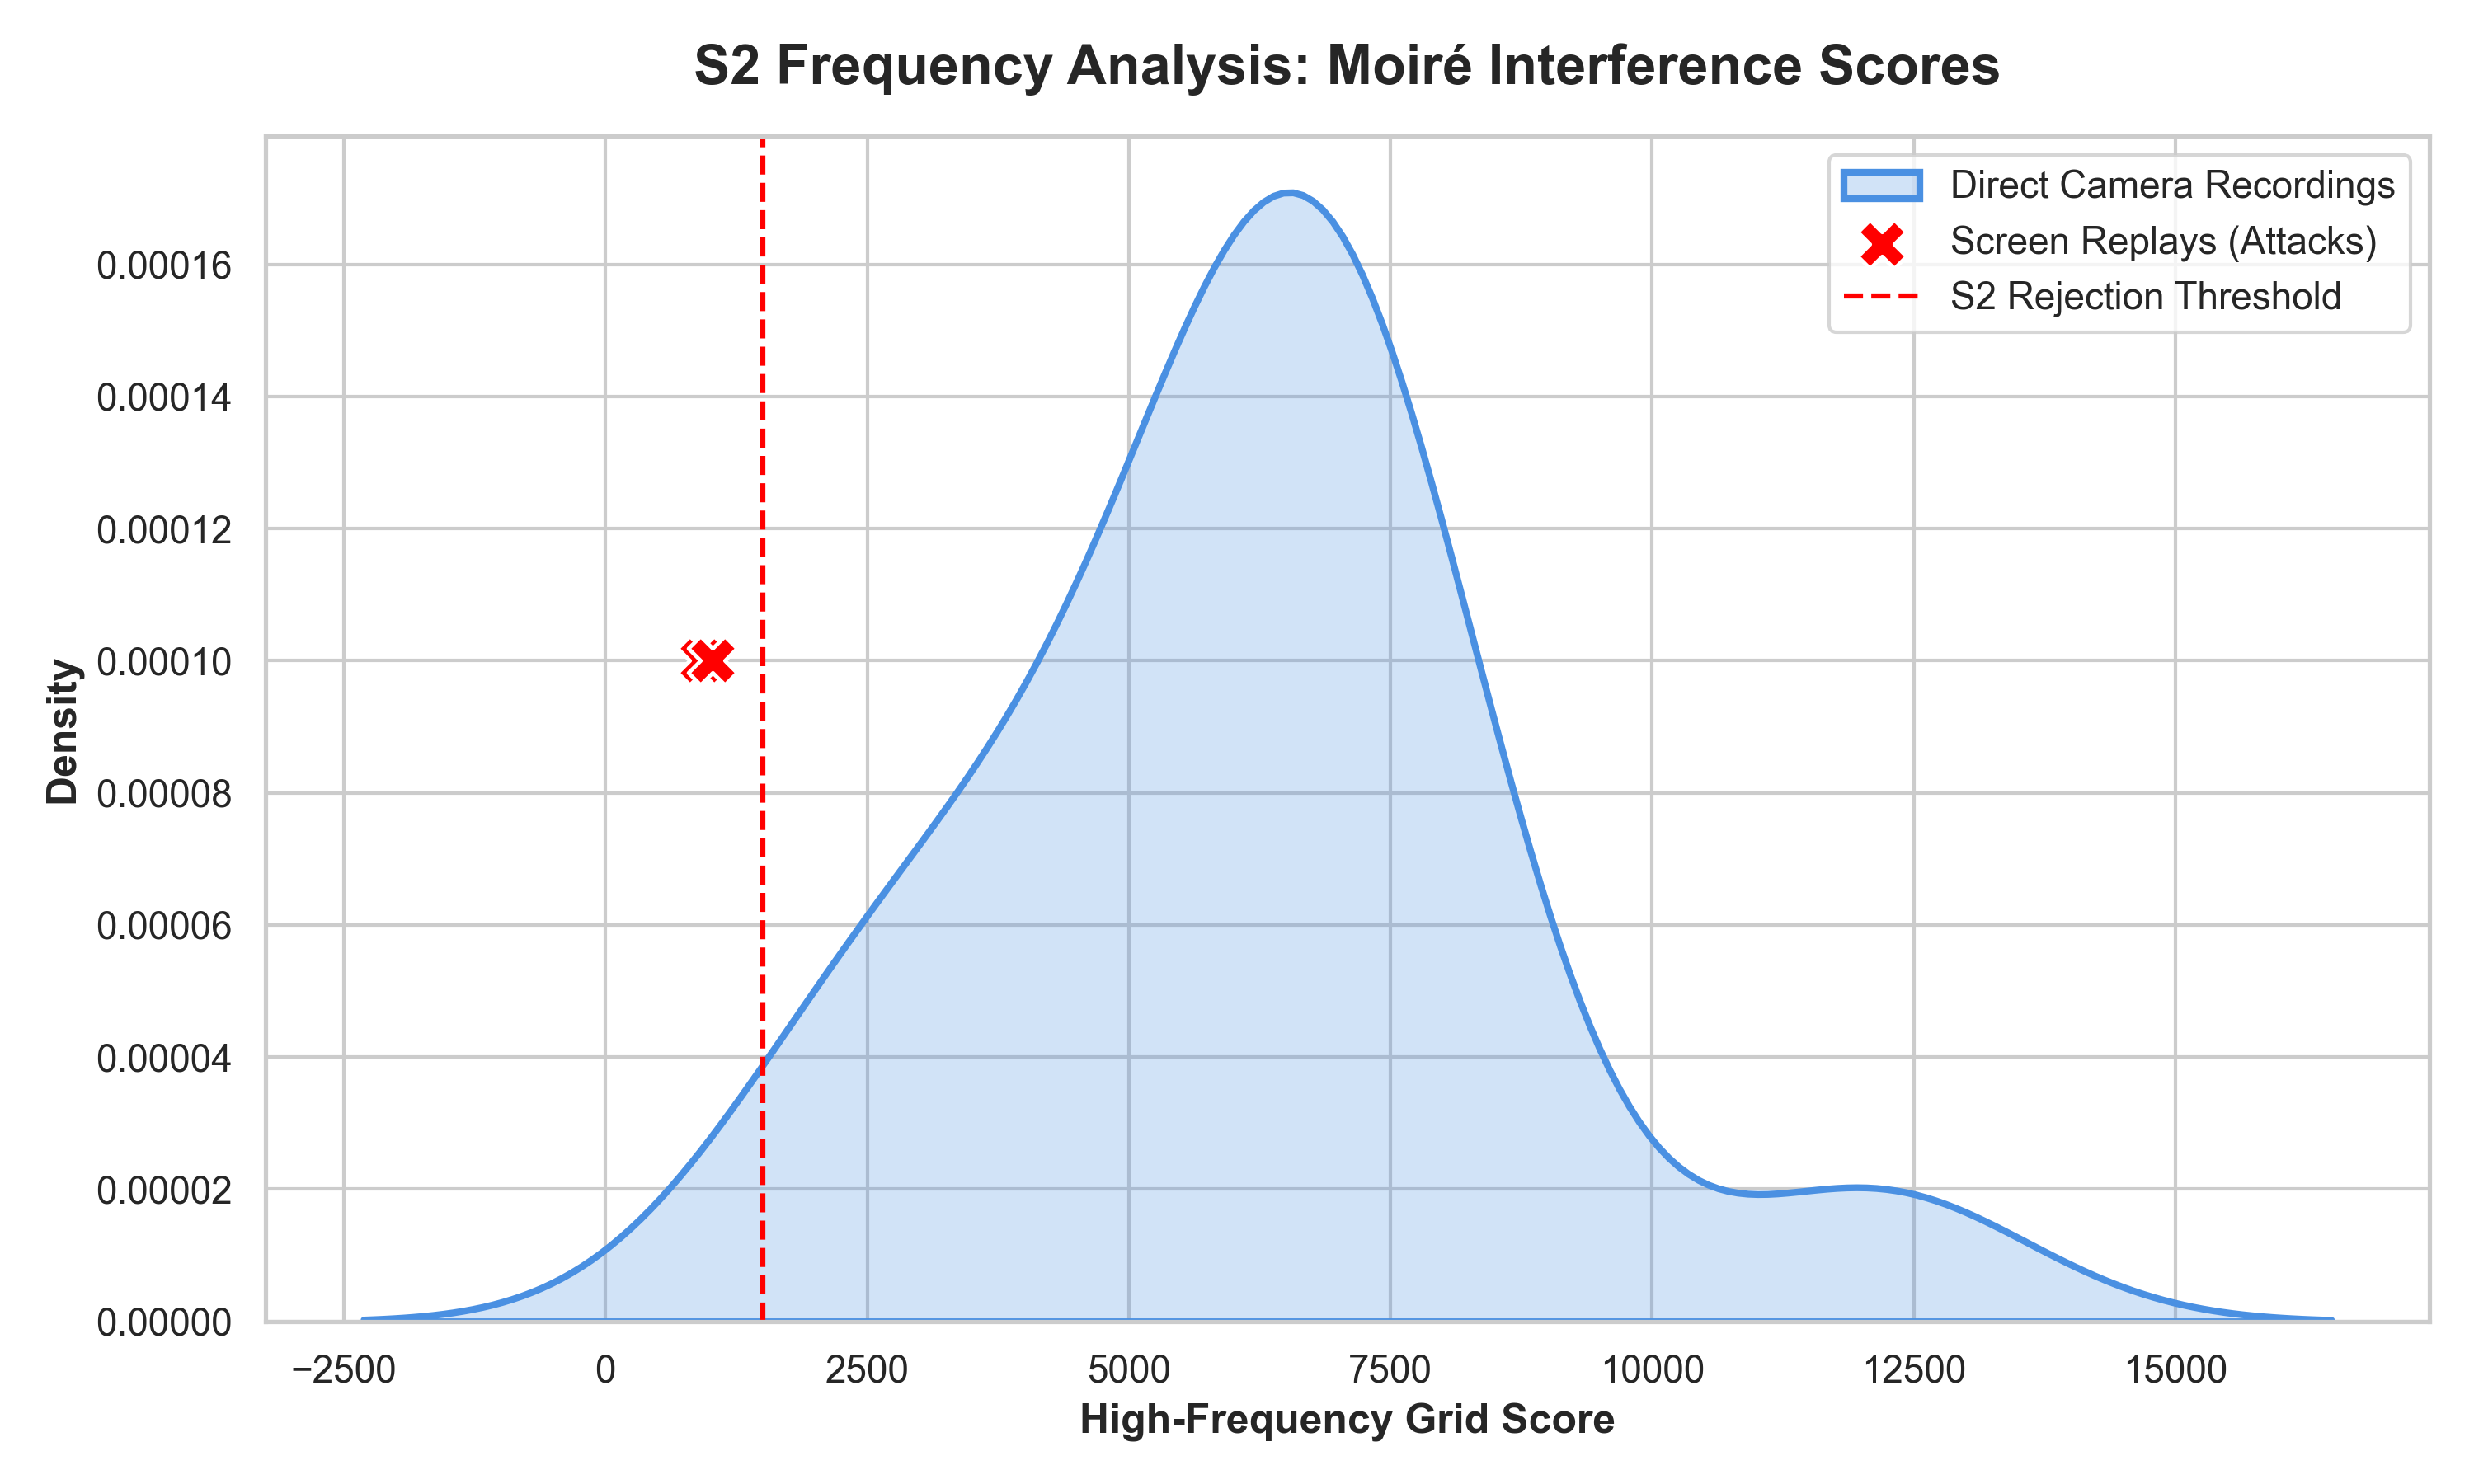
\includegraphics[width=\linewidth]{report_moire_distribution.png}
  \caption{Moiré score distribution. Screen replays cluster at 920--1025; all real camera recordings score above 2,041. The decision boundary at 1500 provides complete mathematical separation.}
  \label{fig:moire_dist}
\end{figure}

Screen replay videos scored 920--1025; real camera recordings scored 2,041--12,135. The threshold at 1500 provides \textbf{complete mathematical separation} with zero overlap.

\subsection{Stage 3: rPPG Biological Liveness}

\textbf{Physical Principle.} Living human skin exhibits sub-visible colour fluctuations driven by the cardiac cycle: haemoglobin absorption modulates reflected light intensity in the green channel ($\approx\!540\,\mathrm{nm}$). Deepfake generators have no incentive to synthesise a coherent cardiovascular pulse waveform.

\textbf{Implementation --- CHROM Algorithm~\cite{dehaan2013}.} MediaPipe Face Mesh (468 landmarks) isolates three skin ROIs (forehead, right cheek, left cheek) via convex hull masks. Per-frame mean R, G, B is extracted; each channel is divided by its temporal mean (AC/DC separation) and linearly detrended to remove auto-exposure drift. The CHROM projection isolates the pulsatile blood volume component:
\begin{align}
  X &= 3R_n - 2G_n - B_n \\
  Y &= 1.5R_n + G_n - 1.5B_n \\
  \text{pulse} &= X - \frac{\sigma_X}{\sigma_Y} \cdot Y
\end{align}
A 4th-order Butterworth IIR filter (0.7--4.0\,Hz; 42--240\,BPM) is applied via \texttt{filtfilt} for zero-phase distortion. Welch's PSD identifies the dominant frequency; SNR is computed as peak power divided by noise floor. Gate logic: $\mathrm{SNR}\geq1.5\,\mathrm{dB}$ AND $45\leq\mathrm{BPM}\leq150 \Rightarrow$ biological liveness confirmed.

\begin{figure}[ht]
  \centering
  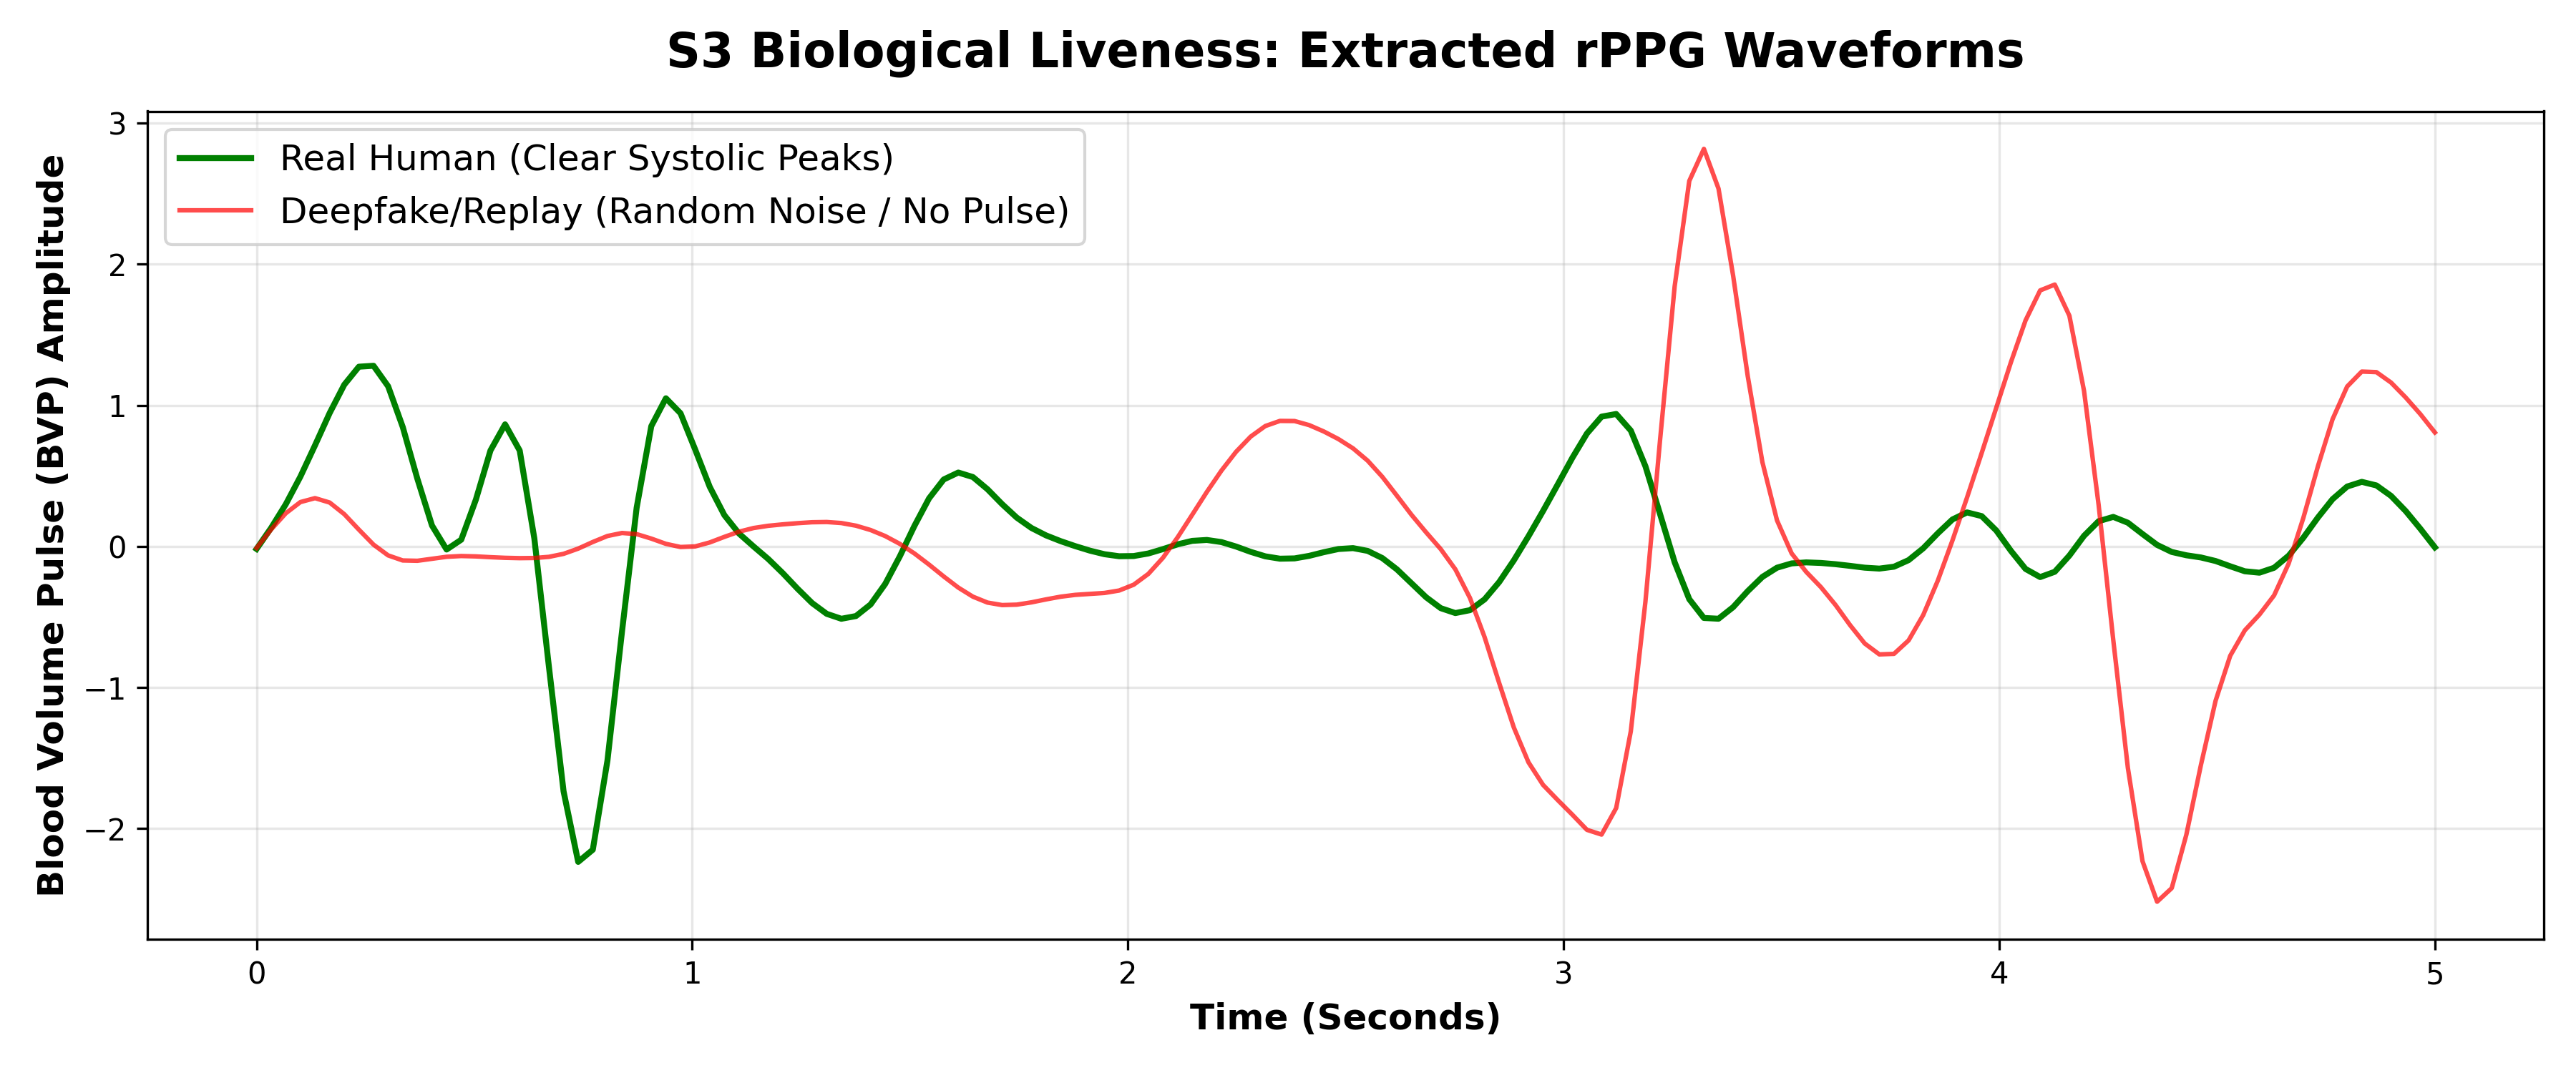
\includegraphics[width=\linewidth]{report_rppg_waveform.png}
  \caption{Extracted Blood Volume Pulse (BVP) waveforms. \emph{Top:} real human showing periodic systolic peaks at $\approx$75\,BPM. \emph{Bottom:} deepfake video yielding only chaotic noise with no discernible cardiac rhythm.}
  \label{fig:rppg}
\end{figure}

\subsection{Stage 4: FTCA --- Frequency-Temporal Cross-Attention}
\label{sec:ftca}

\textbf{Motivation.} Existing detectors operate either spatially (Xception, EfficientNet) or temporally (R3D, SlowFast), but not both. AuthKYC introduces a novel architecture that fuses RGB spatio-temporal features with frequency-domain features through cross-attention, compelling the model to learn \emph{which} frequency artefacts correlate with \emph{which} spatial-temporal movements.

\textbf{RGB Branch.} Input $[B,3,16,224,224]$ (16 contiguous MTCNN-cropped frames) is processed by a pretrained R3D-18~\cite{tran2018} through 4 residual layers of 3D convolutions, producing output $[B,512,2,7,7]$ flattened to a sequence $[B,98,512]$.

\textbf{Frequency Branch.} Per-frame grayscale conversion via luminance weights $(0.2989R + 0.5870G + 0.1140B)$ feeds a differentiable 2D DFT (\texttt{torch.fft.fft2}, orthonormal normalisation). The log-magnitude of the shifted spectrum $\log(|\mathrm{fftshift}(\mathcal{F})| + 10^{-8})$ is encoded by a 4-layer Conv3D encoder (1$\rightarrow$64$\rightarrow$128$\rightarrow$256$\rightarrow$512 channels, matching R3D-18's 8× temporal downsampling), producing $[B,98,512]$.

\textbf{Cross-Attention Fusion.}
\[
  \mathrm{Attn}(Q,K,V) = \mathrm{softmax}\!\left(\frac{QK^\top}{\sqrt{64}}\right) V
\]
where $Q$ = RGB features, $K{=}V$ = frequency features; 8 attention heads, $d_\mathrm{embed}=512$. A residual connection with LayerNorm follows: $\mathrm{out} = \mathrm{LN}(f_\mathrm{RGB} + \mathrm{attn\_out})$.

\textbf{Classifier.} AdaptiveAvgPool1d(1) $\rightarrow$ Linear(512$\rightarrow$128) $\rightarrow$ ReLU $\rightarrow$ Dropout(0.5) $\rightarrow$ Linear(128$\rightarrow$1). Sigmoid output $> 0.50 \Rightarrow$ deepfake.

\begin{figure}[ht]
  \centering
  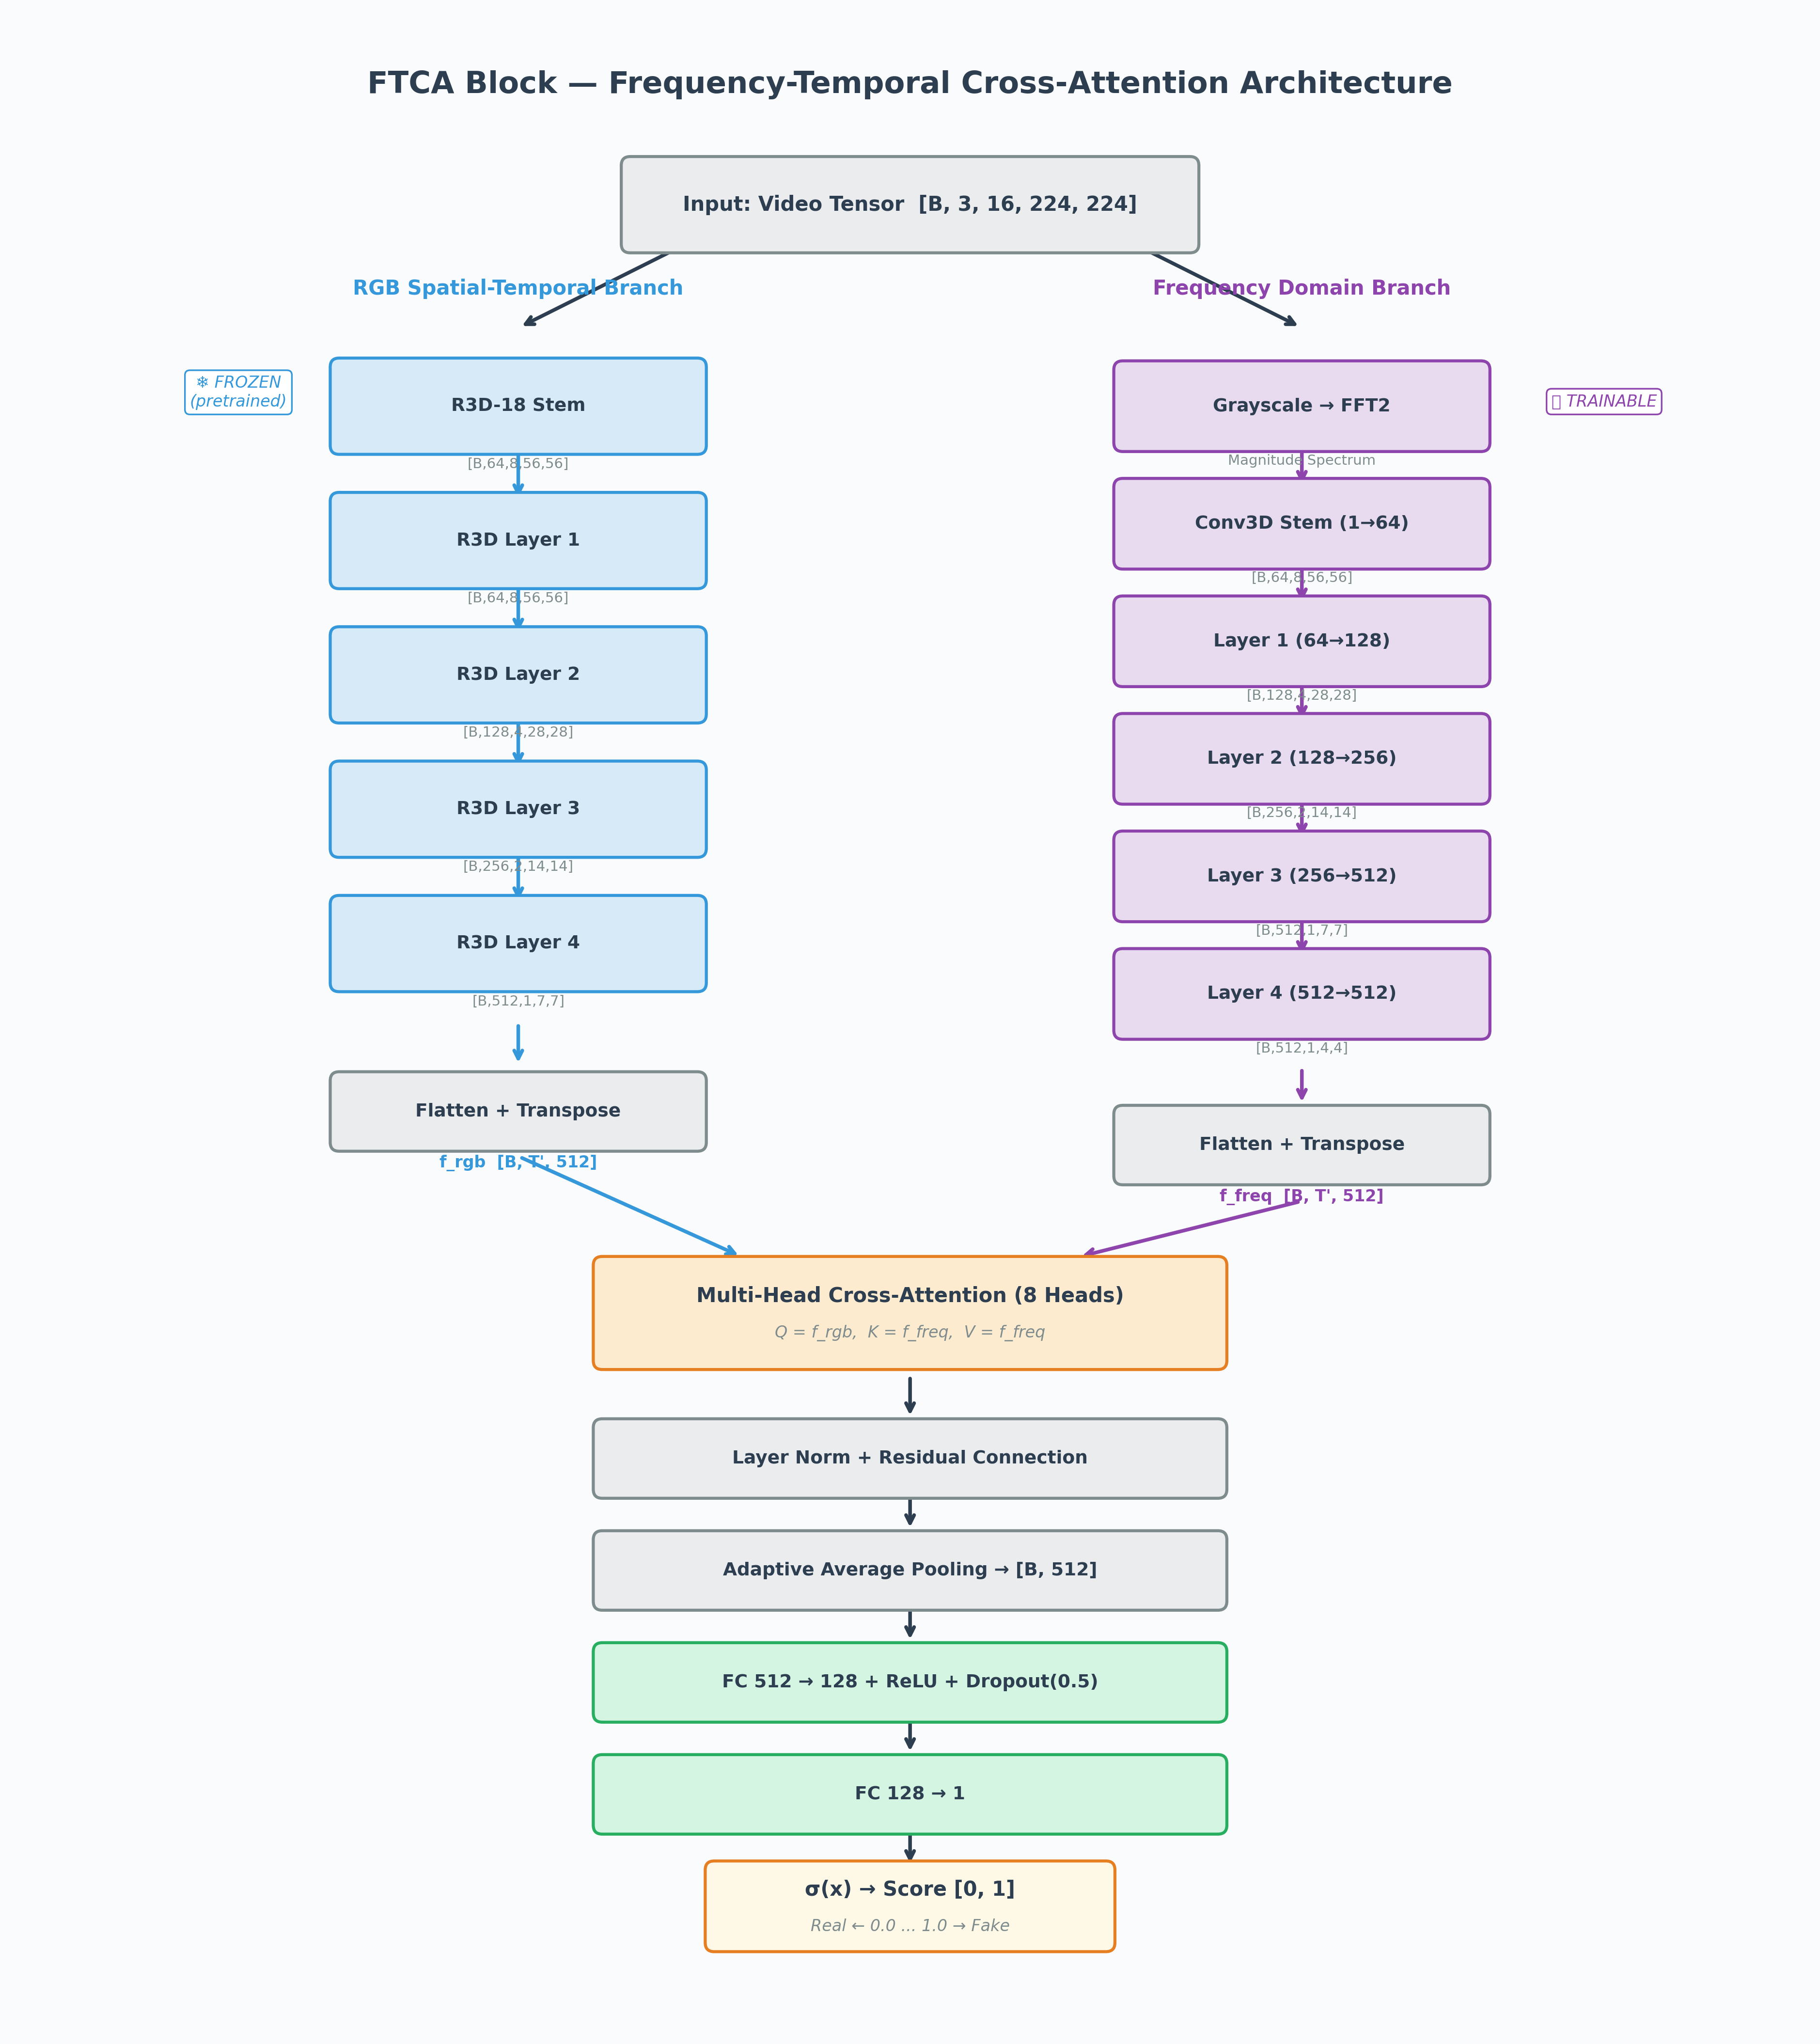
\includegraphics[width=\linewidth]{ftca_block_diagram.png}
  \caption{FTCA block diagram. RGB and frequency branches process the same 16-frame clip in parallel; multi-head cross-attention fuses their representations before the binary classifier.}
  \label{fig:ftca}
\end{figure}

\subsection{Dynamic Fallback Routing}
\label{sec:fallback}

Modern smartphones apply aggressive Electronic Image Stabilisation (EIS) and temporal denoising that destroy the S1 PRNU fingerprint. Without mitigation, every legitimate phone KYC session would be falsely rejected. The solution: if S1 fails but the system detects a verified biological heartbeat (S3 pass) AND zero AI manipulation (S4 pass), biological and AI evidence overrides the hardware failure:

\begin{lstlisting}
if not s1_prnu_pass and s3_rppg_pass and s4_ftca_pass:
    s1_pass = True  # Dynamic Override
\end{lstlisting}

An attacker must simultaneously fake a biological pulse \emph{and} pass the FTCA deepfake detector to exploit this override, ensuring security is not compromised.

% ============================================================
\section{Training Pipeline}
\label{sec:training}

\subsection{Dataset and Extraction}

Training data comprised FaceForensics++ C23~\cite{rossler2019} (original + 5 manipulation methods: Deepfakes, Face2Face, FaceSwap, FaceShifter, DeepFakeDetection) and Celeb-DF v2~\cite{li2020}. A balanced 1500 real + 1500 fake split (seed=42, 80/20 train/val) was used. MTCNN~\cite{zhang2016} detected and cropped faces to $224\times224$ (40\,px margin); up to 8 contiguous 16-frame sequences were extracted per video.

\subsection{Phase 1: Full FTCA Training}

\begin{table}[ht]
\centering
\caption{Phase 1 Training Hyperparameters (Full FTCA)}
\label{tab:train1}
\renewcommand{\arraystretch}{1.1}
\begin{tabular}{@{}ll@{}}
\toprule
\textbf{Parameter} & \textbf{Value} \\ \midrule
Architecture & FTCABlock (R3D-18 + FreqEncoder + CrossAttn) \\
Parameters & $\approx$12.8M \\
Optimiser & AdamW (lr=$10^{-4}$, wd=$10^{-3}$) \\
Scheduler & ReduceLROnPlateau (factor=0.5, patience=3) \\
Loss & BCEWithLogitsLoss \\
Precision & Mixed (AMP + GradScaler) \\
Batch Size & 16 \\
Epochs & 30 \\
Hardware & NVIDIA RTX A6000 (48\,GB) via RunPod \\
\textbf{Best Val Acc} & \textbf{64.67\%} \\
\textbf{Best Val Loss} & \textbf{0.6053} \\ \bottomrule
\end{tabular}
\end{table}

\begin{figure}[ht]
  \centering
  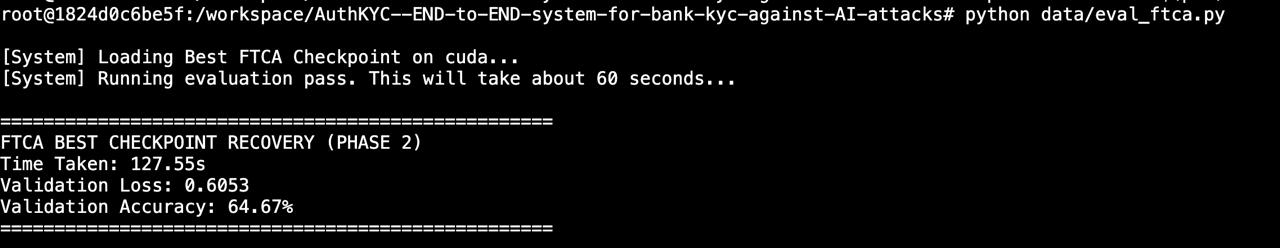
\includegraphics[width=\linewidth]{fcta_train1.jpeg}
  \caption{Phase 1 training curves: validation accuracy and loss across 30 epochs.}
  \label{fig:train1}
\end{figure}

\subsection{Phase 2: Xception Baseline}

To establish that temporal analysis is necessary, we trained an Xception~\cite{chollet2017} baseline using the \texttt{timm} library ($\approx$22M parameters, pretrained ImageNet, Adam lr=$10^{-4}$, 20 epochs, best val accuracy: 46.92\%). Xception's validation loss diverged from training loss after epoch 5 --- classic overfitting to spatial compression artefacts rather than genuine deepfake features.

\begin{figure}[ht]
  \centering
  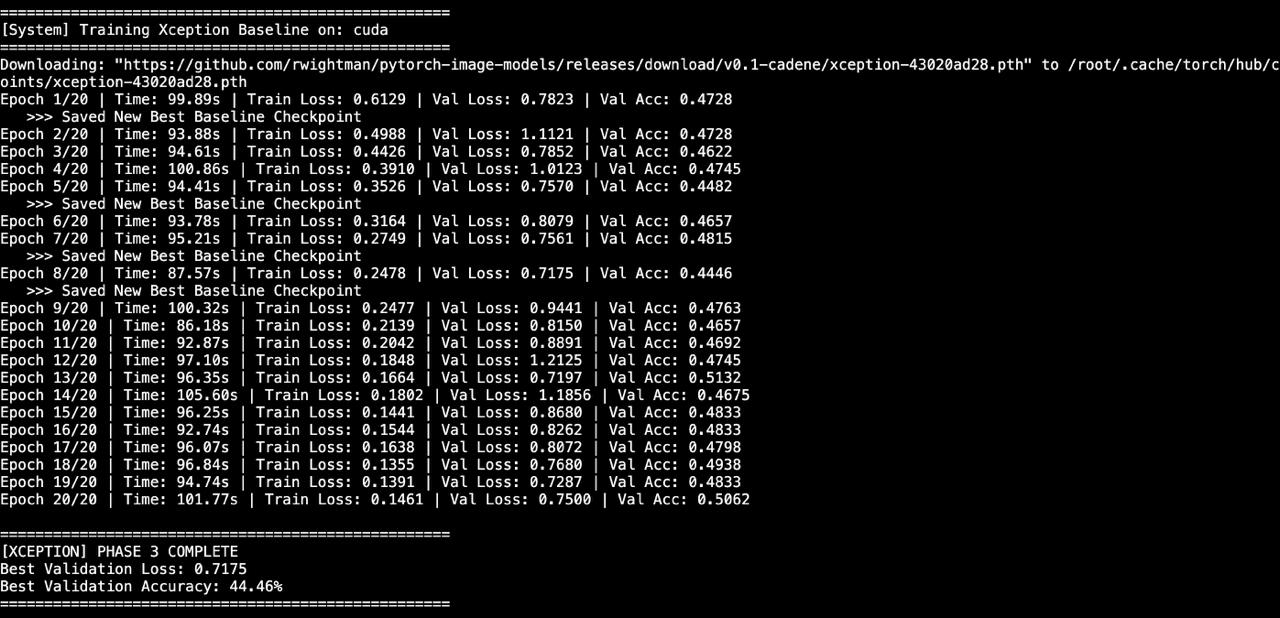
\includegraphics[width=\linewidth]{xception_baseline.jpeg}
  \caption{Xception baseline training curves showing clear overfitting after epoch 5.}
  \label{fig:xception}
\end{figure}

\subsection{Phase 3: Domain Adaptation Fine-Tuning}

To close the domain gap between FF++ training data and real-world webcam/phone footage, targeted fine-tuning was performed on a custom dataset: 250 webcam anchor videos (real recordings augmented via HFlip, ColorJitter, GaussianBlur), 250 FF++ original videos, and 500 FF++ fake videos. The entire R3D-18 backbone was frozen; only the FrequencyEncoder, CrossAttention, LayerNorm, and Classifier ($\approx$5.2M parameters) were trained (AdamW lr=$10^{-5}$, 15 epochs).

\begin{figure}[ht]
  \centering
  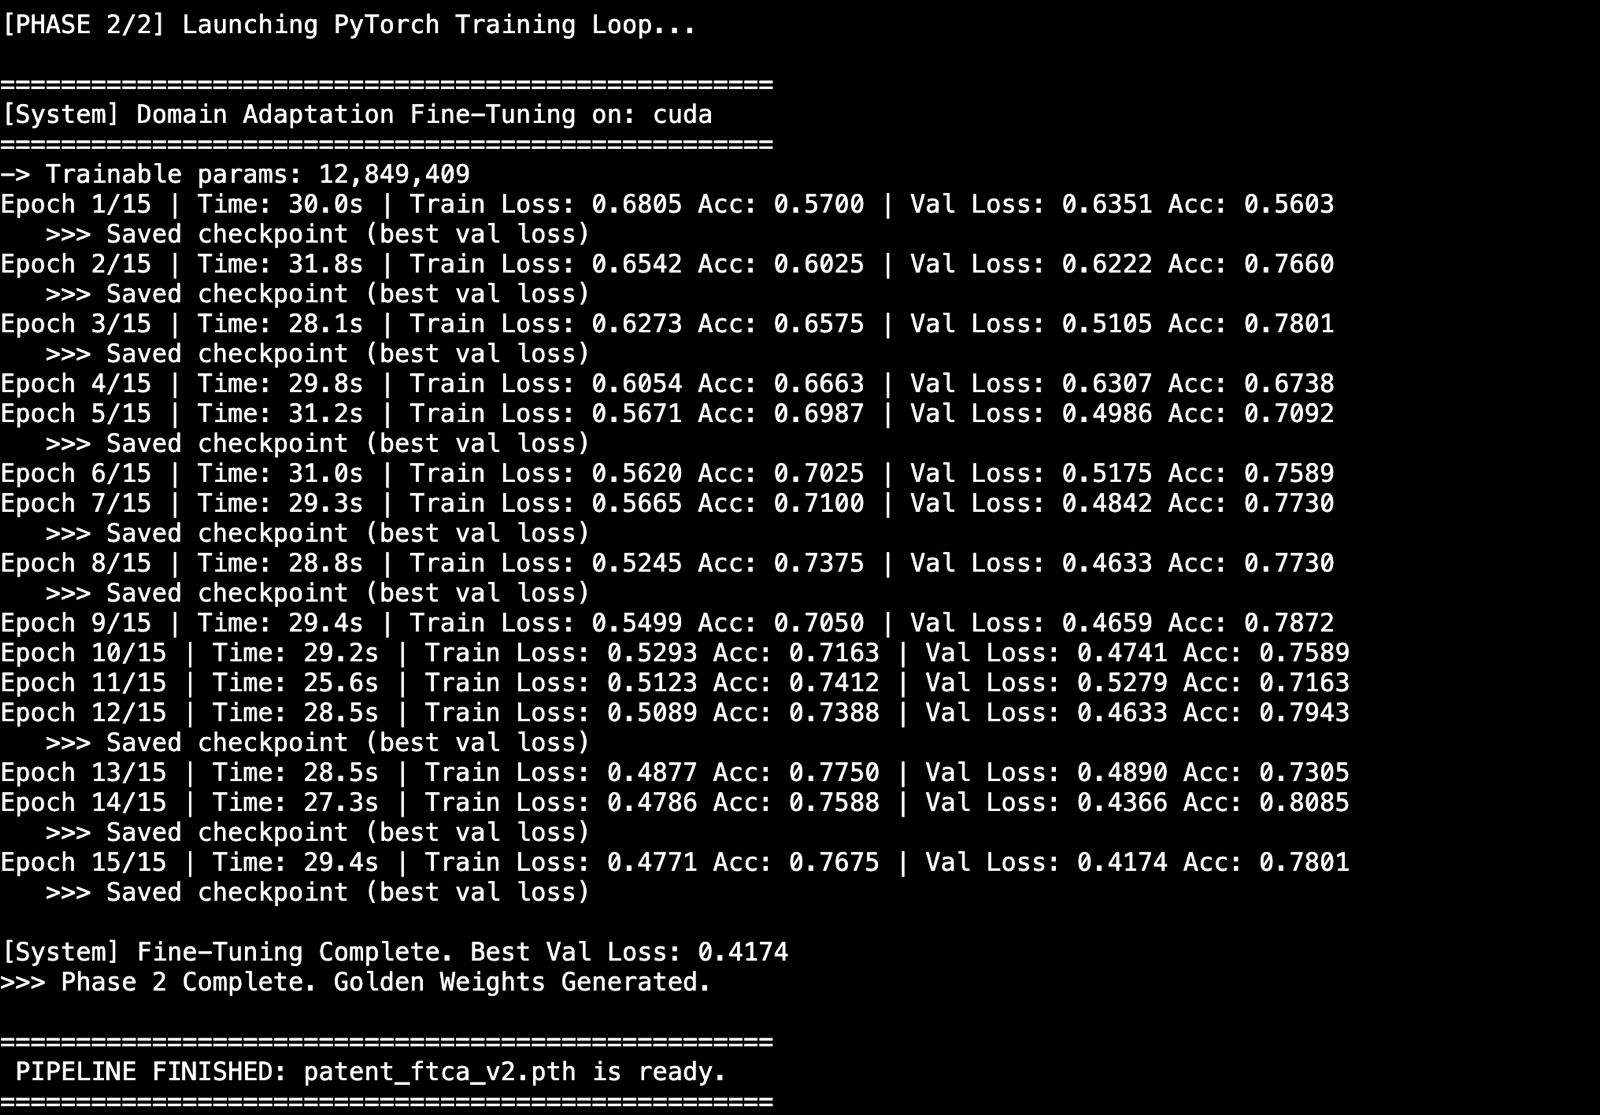
\includegraphics[width=\linewidth]{ftca_finetune.jpeg}
  \caption{Phase 3 fine-tuning curves. Domain adaptation improves validation accuracy from 64.67\% to 80.85\%.}
  \label{fig:finetune}
\end{figure}

\begin{figure}[ht]
  \centering
  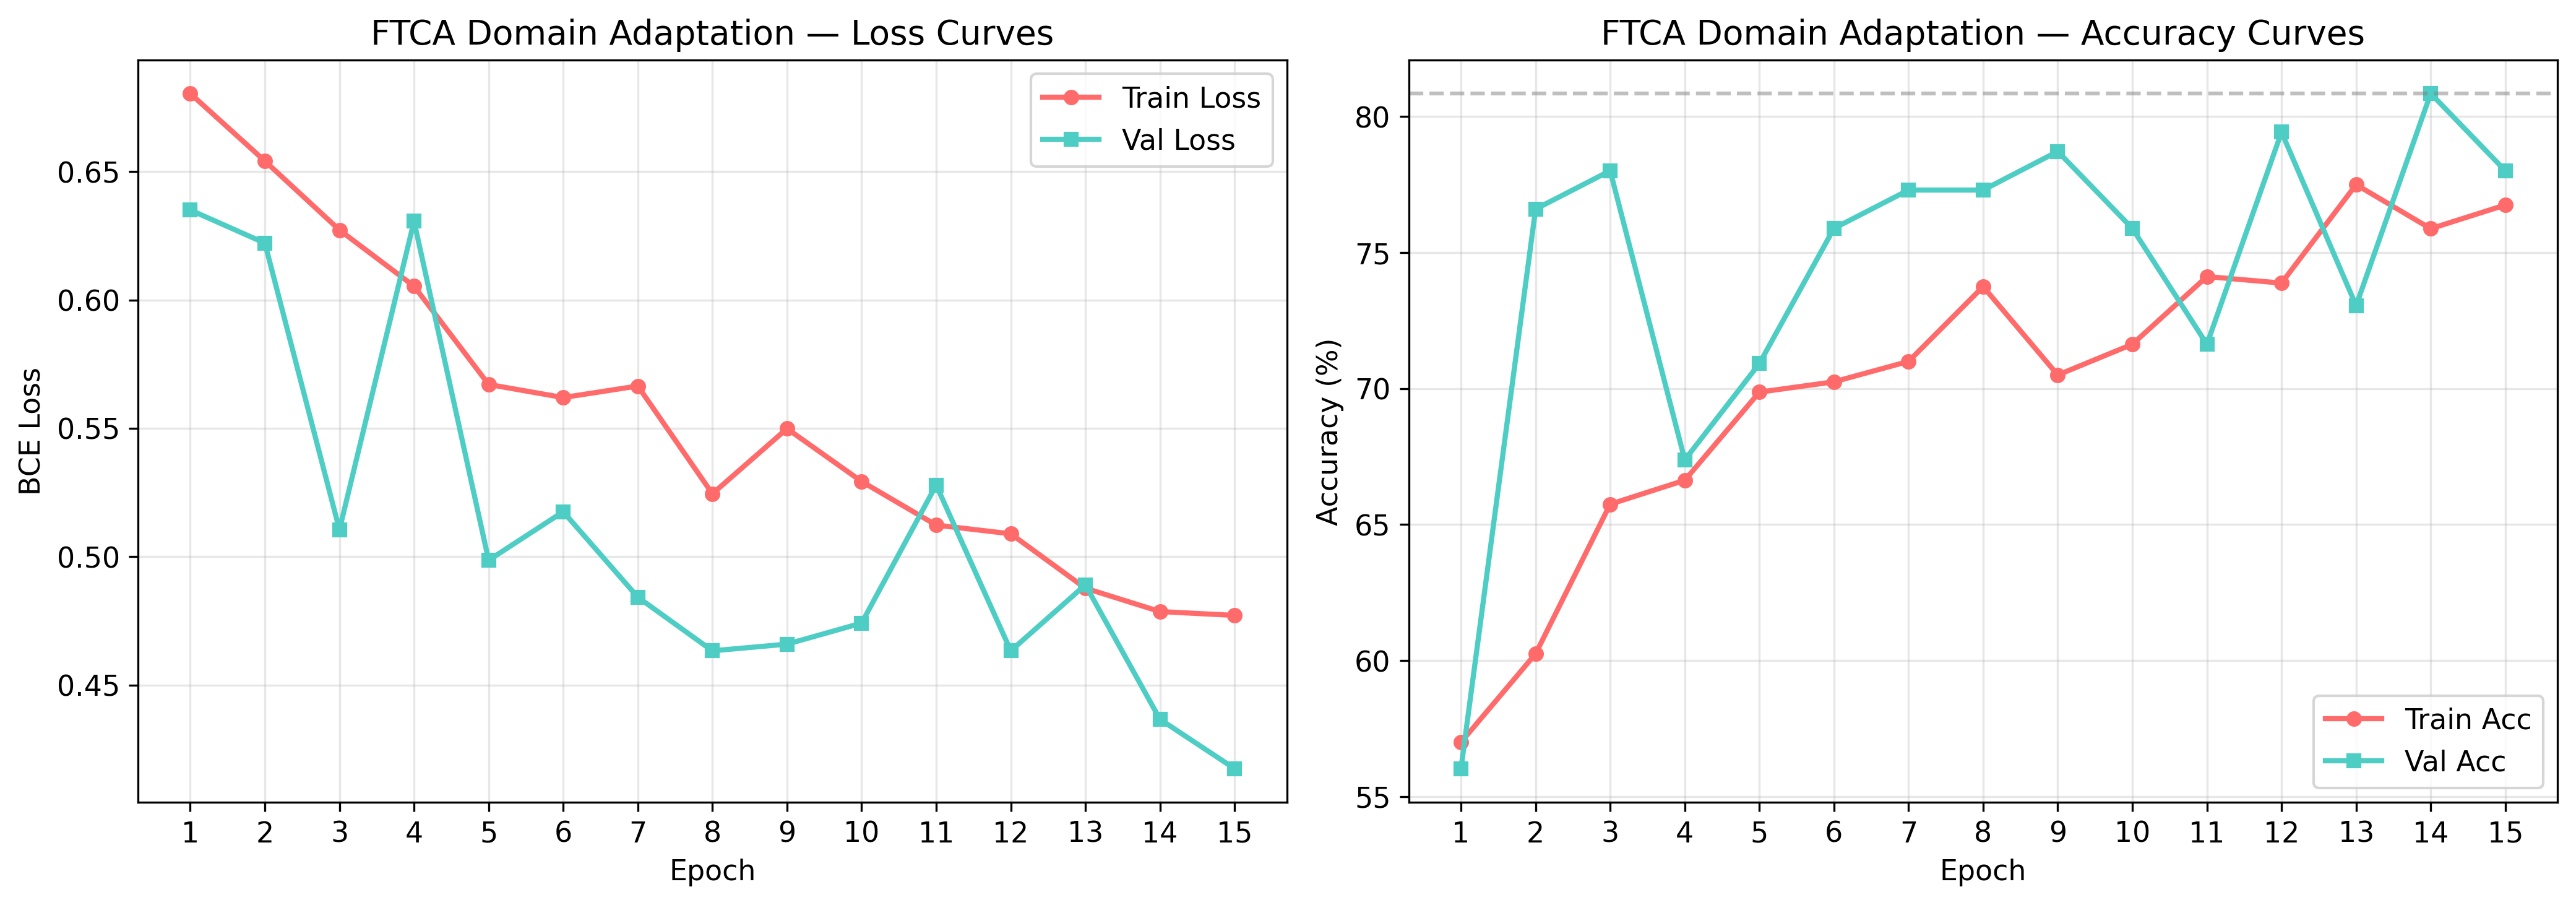
\includegraphics[width=\linewidth]{fig1_ftca_training_curves.png}
  \caption{Aggregated FTCA training and fine-tuning curves.}
  \label{fig:allcurves}
\end{figure}

% ============================================================
\section{Experimental Results}
\label{sec:results}

\subsection{End-to-End Waterfall Evaluation (Experiment 6)}

\textbf{Dataset ($N=21$):} 12 real human videos (4 FF++ C23 originals + 8 uncompressed mobile recordings under varying lighting), 2 physical screen-replay attacks (phone screen held to MacBook webcam), and 7 FF++ C23 deepfakes (Deepfakes and Face2Face methods). Including compressed FF++ ``Real'' videos alongside uncompressed mobile recordings was a deliberate experimental control: if FTCA were learning the domain gap rather than genuine artefacts, these videos would have been misclassified. Their successful passage confirms the model evaluates spatio-temporal blending artefacts.

\begin{table}[ht]
\centering
\caption{End-to-End Waterfall Results ($N=21$)}
\label{tab:results}
\renewcommand{\arraystretch}{1.1}
\begin{tabular}{@{}lccr@{}}
\toprule
\textbf{Category} & \textbf{Total} & \textbf{Correct} & \textbf{Accuracy} \\ \midrule
Real Humans (Approval Rate) & 12 & 11 & 91.7\% \\
Screen Replays (Detection) & 2 & 2 & 100.0\% \\
Deepfakes FF++ (Detection) & 7 & 7 & 100.0\% \\
\midrule
\textbf{Overall} & \textbf{21} & \textbf{20} & \textbf{95.2\%} \\
\bottomrule
\end{tabular}
\end{table}

\begin{table}[ht]
\centering
\caption{Confusion Matrix}
\label{tab:conf}
\renewcommand{\arraystretch}{1.15}
\begin{tabular}{@{}lcc@{}}
\toprule
& \textbf{Pred. PASS} & \textbf{Pred. REJECT} \\ \midrule
\textbf{Actual Real} & TP = 11 & FN = 1 \\
\textbf{Actual Attack} & FP = 0 & TN = 9 \\ \bottomrule
\end{tabular}
\end{table}

\textbf{False Positive Rate: 0\%} --- no attack of any type bypassed the waterfall.

\begin{figure}[ht]
  \centering
  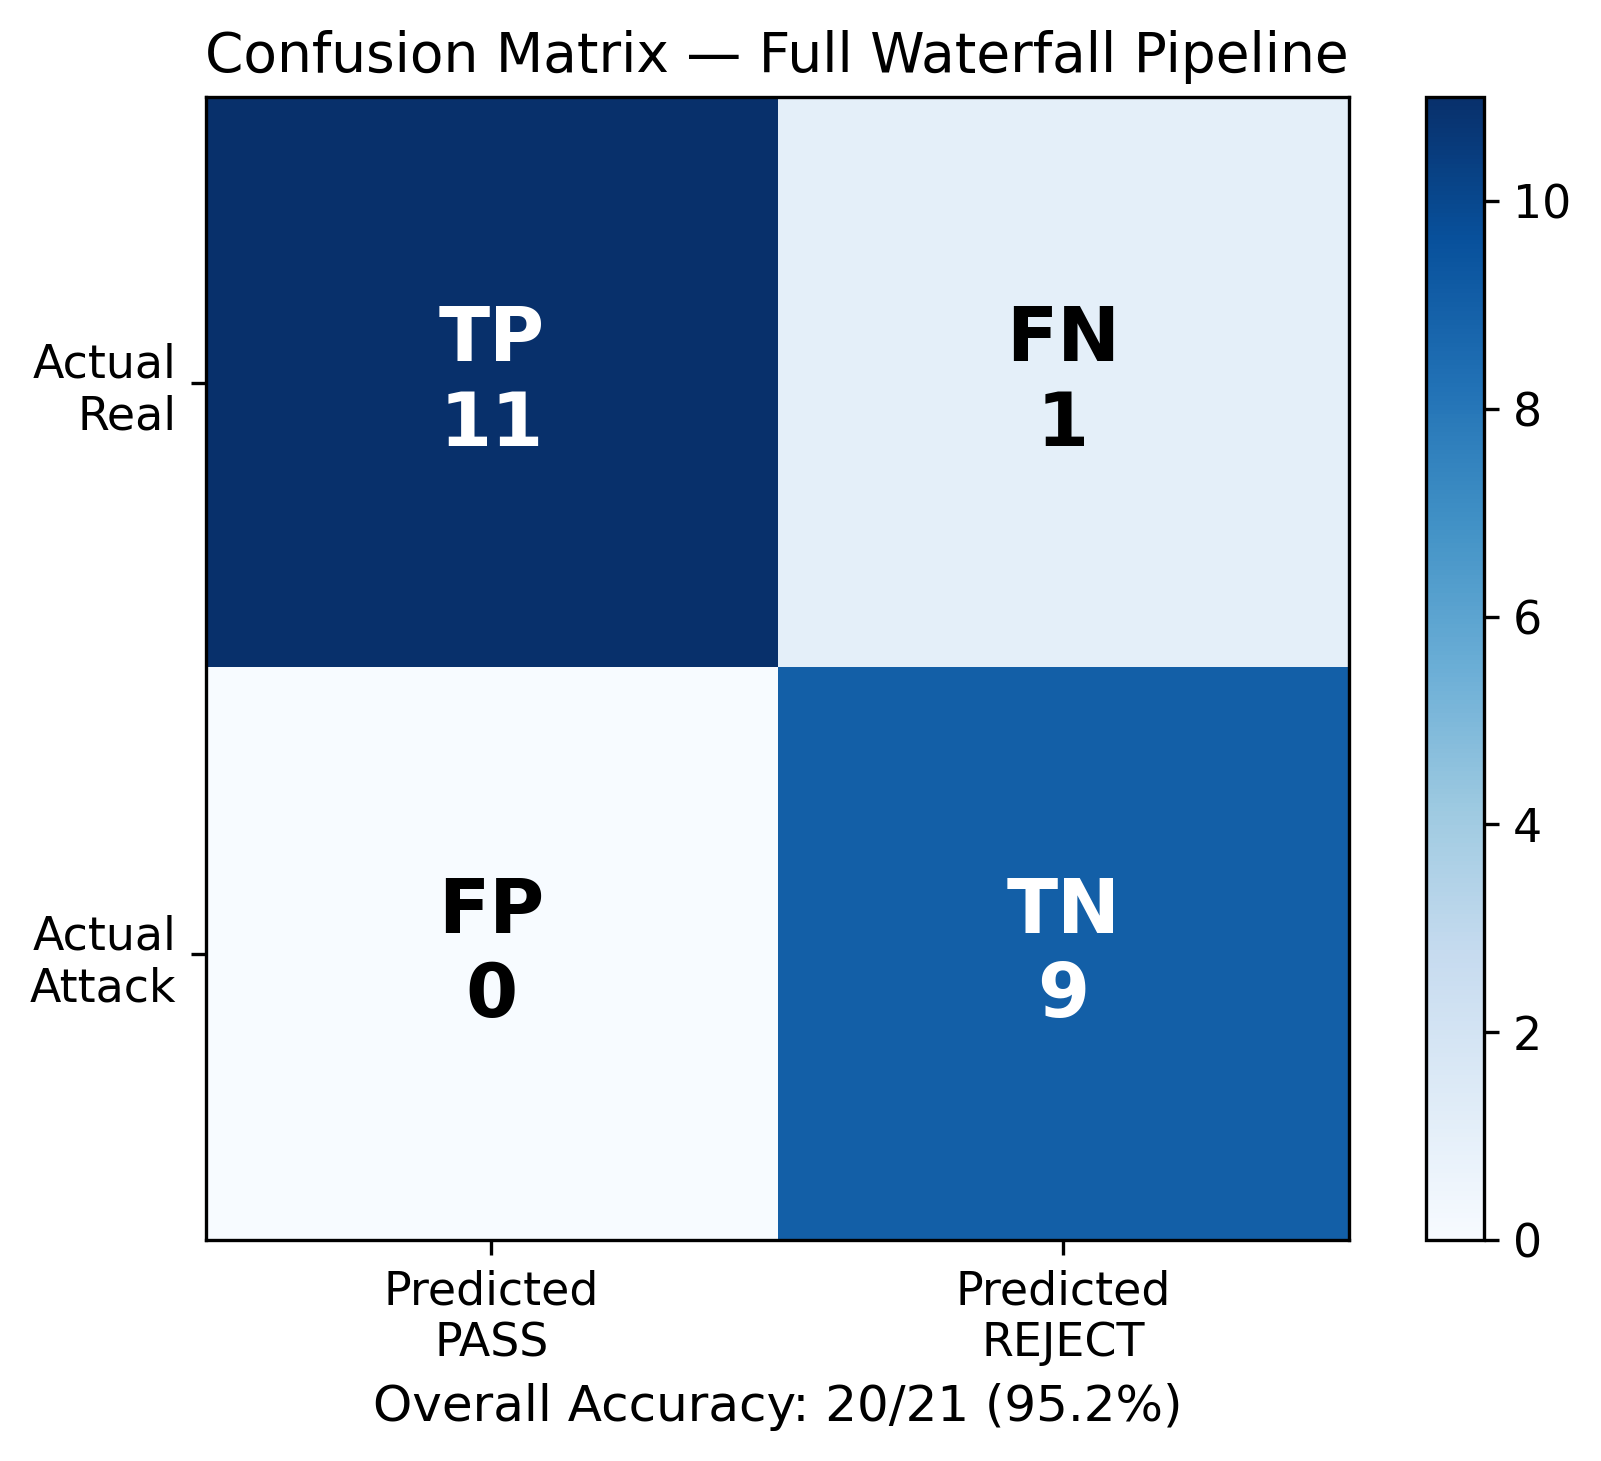
\includegraphics[width=\linewidth]{fig3_confusion_matrix.png}
  \caption{Confusion matrix on the 21-video mixed-domain evaluation set.}
  \label{fig:conf}
\end{figure}

\textbf{Defence-in-Depth.} Table~\ref{tab:waterfall} shows which stage intercepted each attack. A critical finding: screen replay attacks scored as ``real'' by S4 (they contain genuine face textures), confirming that the physical S2 layer is indispensable.

\begin{table}[ht]
\centering
\caption{Per-Stage Attack Attribution}
\label{tab:waterfall}
\renewcommand{\arraystretch}{1.1}
\begin{tabular}{@{}lcc@{}}
\toprule
\textbf{Stage} & \textbf{Attacks Caught} & \textbf{Attack Types} \\ \midrule
S2 (Moiré) & 3 & 2 replays + 1 compressed deepfake \\
S3 (rPPG) & 1 & Deepfake with no detectable pulse \\
S4 (FTCA) & 5 & Software deepfakes passing S2/S3 \\
Escaped & 0 & --- \\ \bottomrule
\end{tabular}
\end{table}

\begin{figure}[ht]
  \centering
  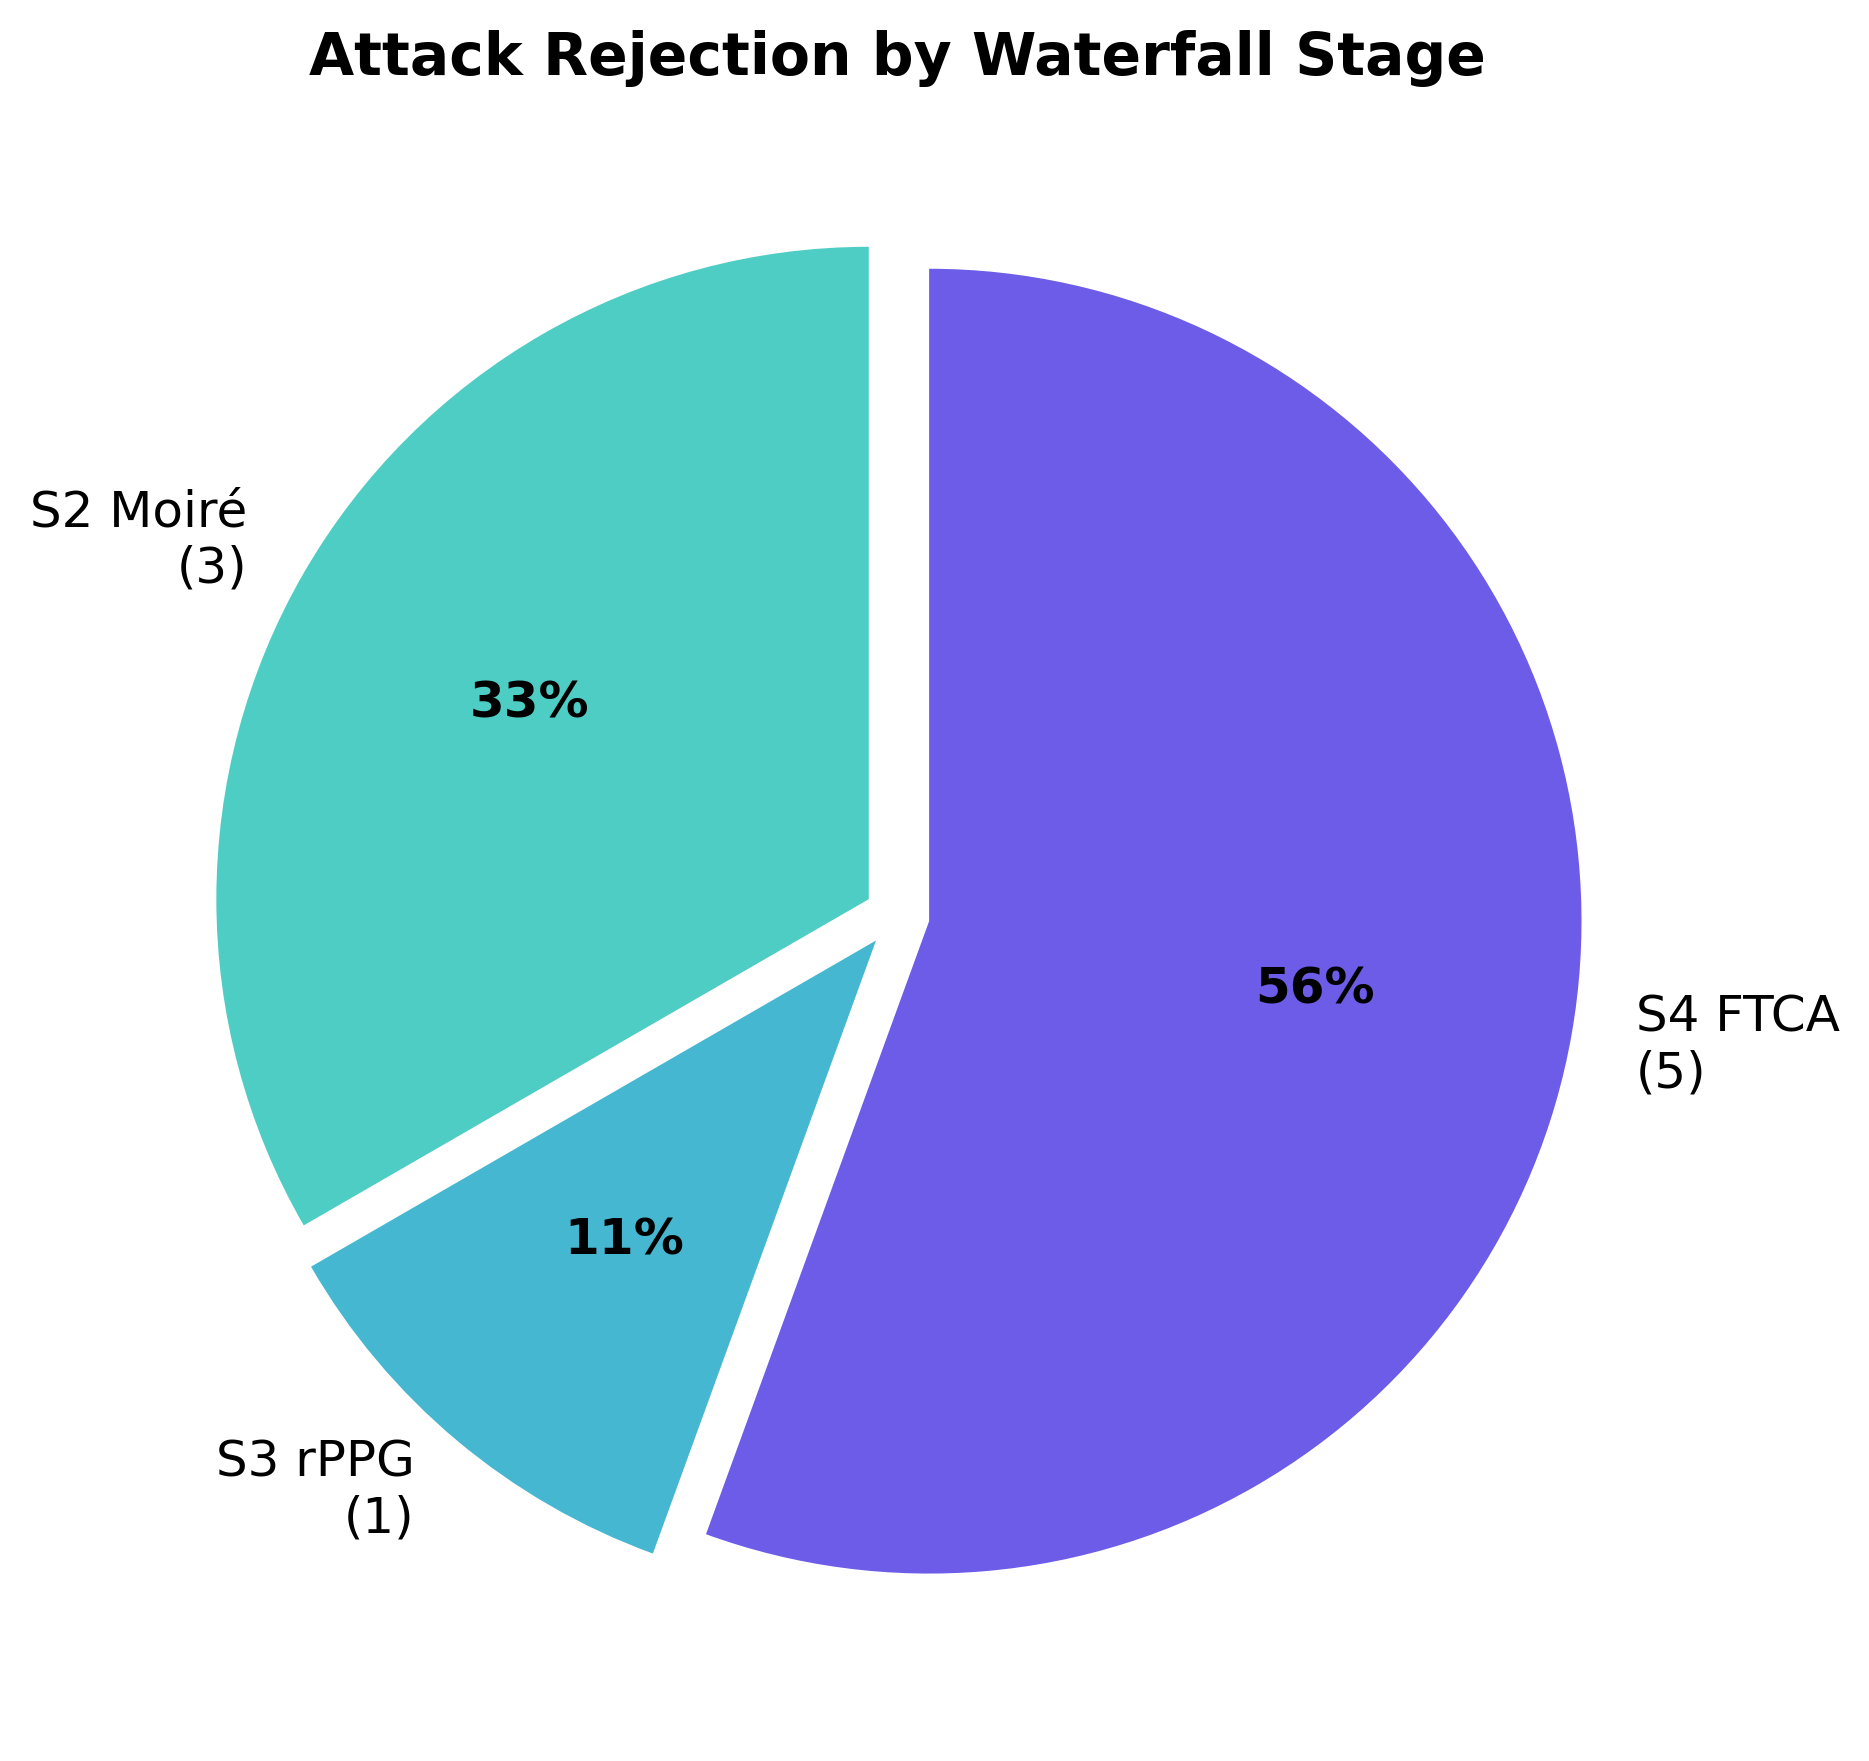
\includegraphics[width=\linewidth]{fig4_waterfall_rejection.png}
  \caption{Waterfall rejection diagram showing which stage intercepted each attack class.}
  \label{fig:waterfall}
\end{figure}

\subsection{Signal-Level Visualisations}

Figure~\ref{fig:ftca_scores} shows FTCA score distributions: real videos score 0.017--0.294 (one outlier at 0.781); deepfakes score 0.614--0.800; screen replays score 0.024--0.040 (correctly classified by S2 \emph{before} reaching S4).

\begin{figure}[ht]
  \centering
  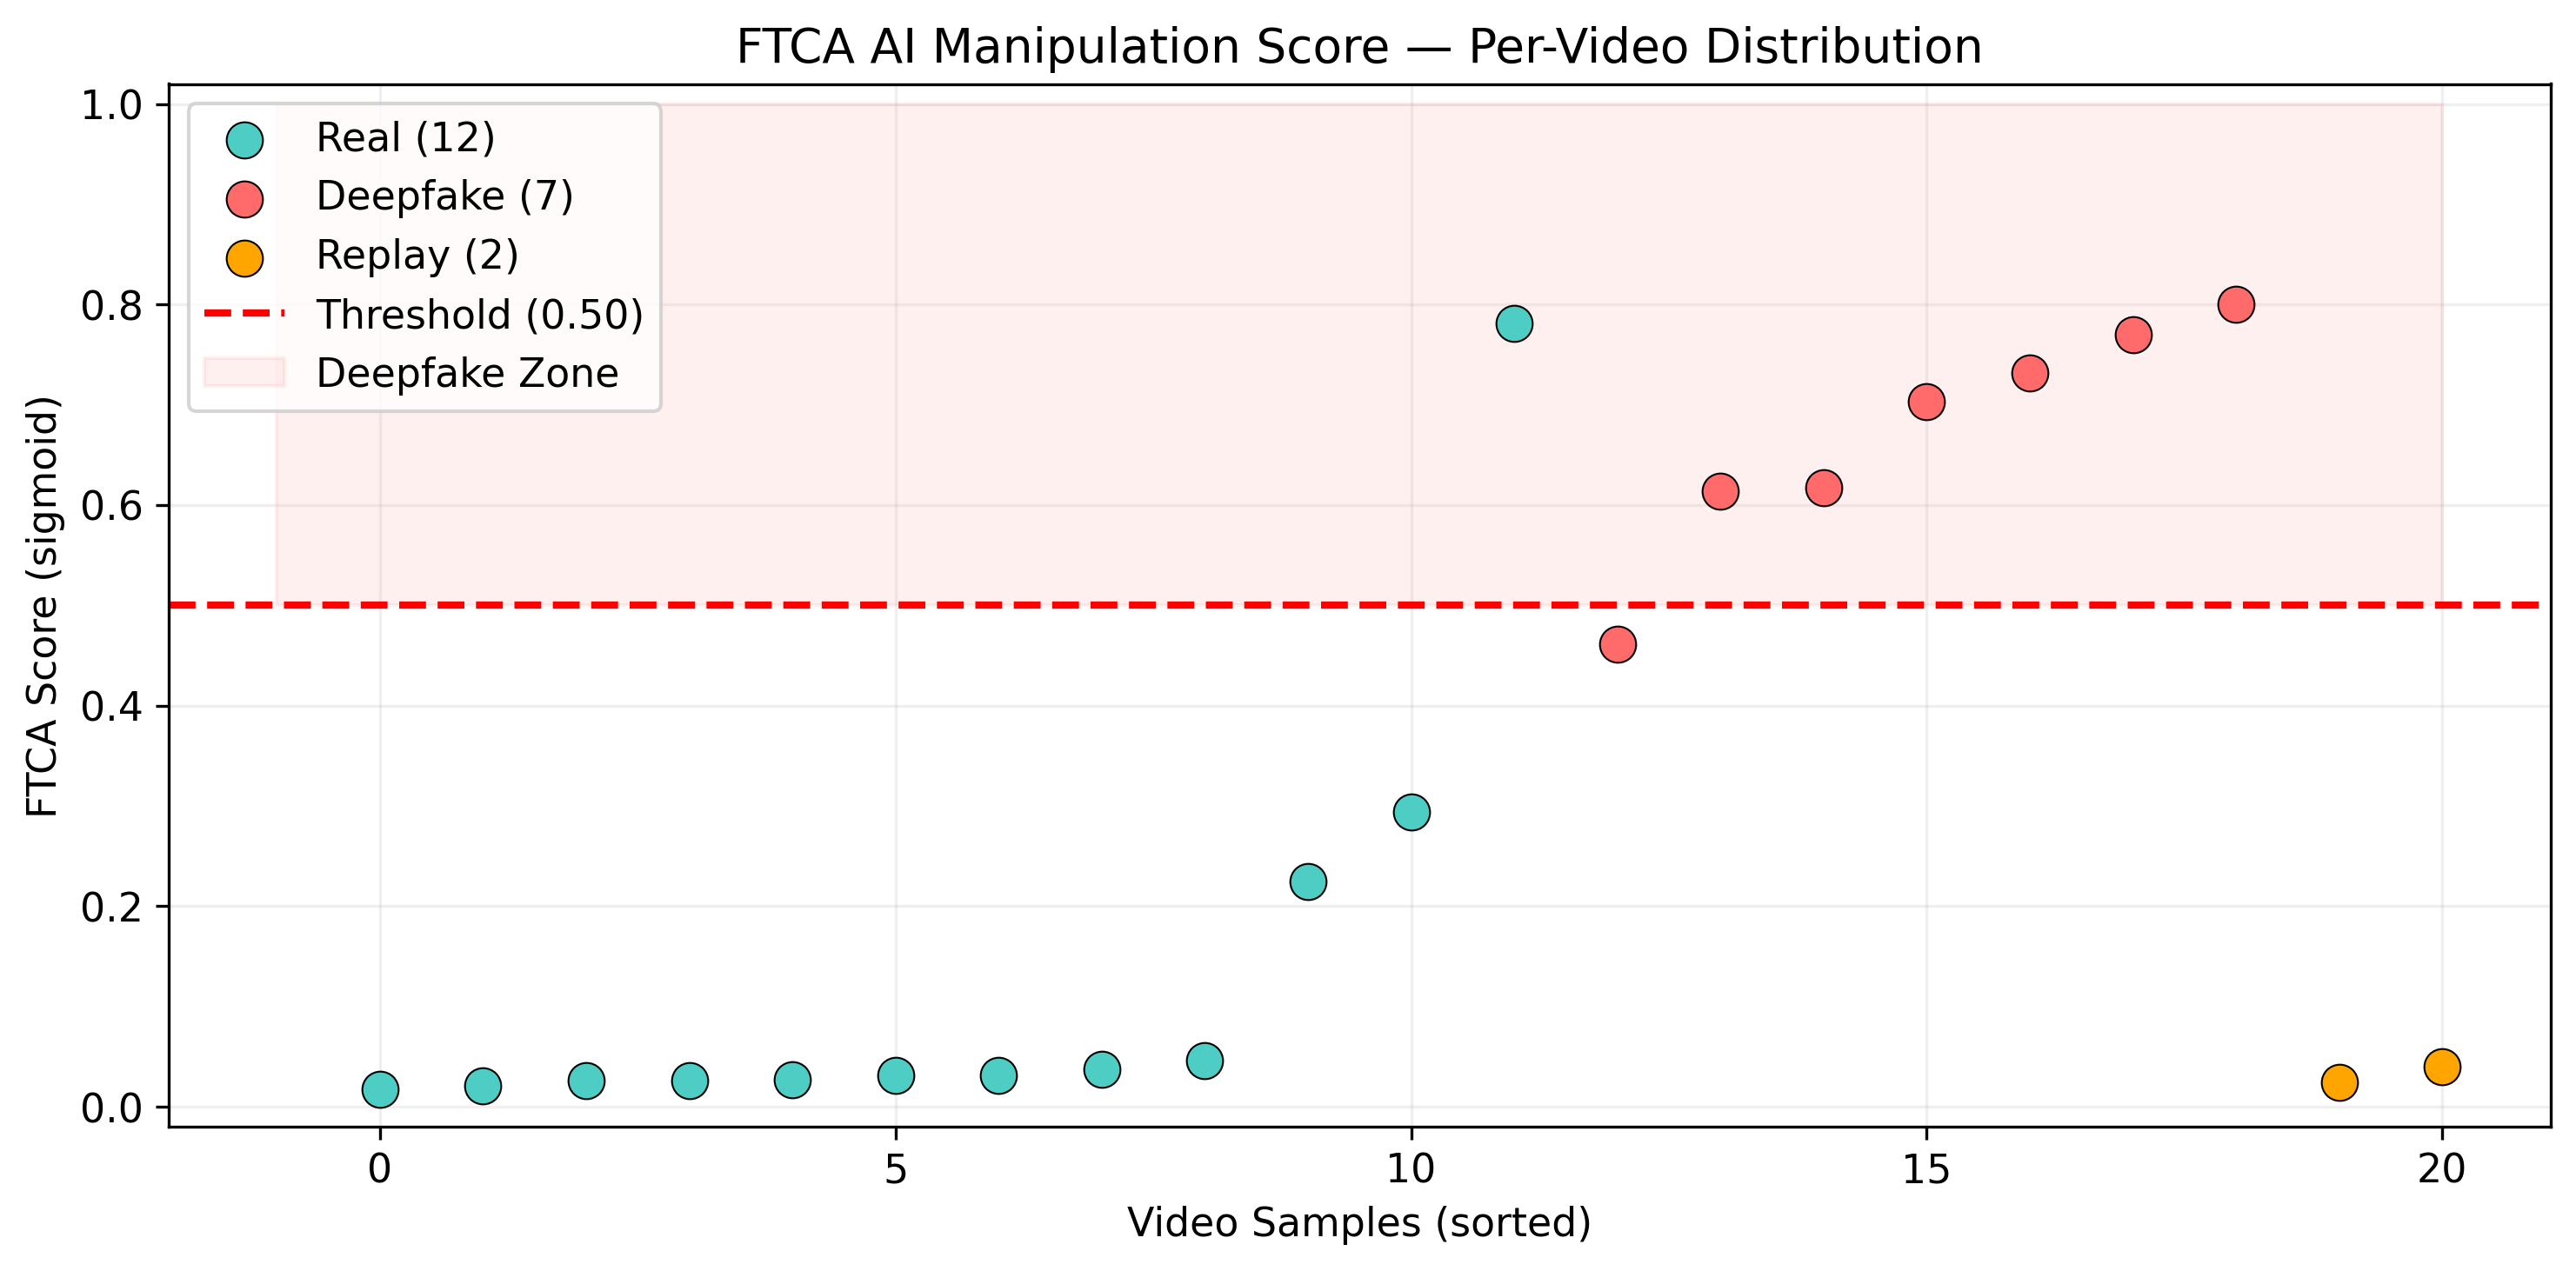
\includegraphics[width=\linewidth]{fig6_ftca_score_distribution.png}
  \caption{FTCA sigmoid score distributions. Real and deepfake populations are well-separated around the 0.50 decision threshold. Screen replays score near zero (genuine textures), confirming S2 must precede S4.}
  \label{fig:ftca_scores}
\end{figure}

\subsection{Model Comparison}

\begin{table}[ht]
\centering
\caption{Model Comparison}
\label{tab:models}
\renewcommand{\arraystretch}{1.1}
\begin{tabular}{@{}lcccc@{}}
\toprule
\textbf{Model} & \textbf{Val Acc} & \textbf{Val Loss} & \textbf{Params} & \textbf{Temporal} \\ \midrule
\textbf{FTCA (fine-tuned)} & \textbf{80.85\%} & \textbf{0.4174} & 12.8M & Yes \\
FTCA (pretrained only) & 64.67\% & 0.6053 & 12.8M & Yes \\
Xception Baseline & 46.92\% & 0.6940 & $\approx$22M & No \\ \bottomrule
\end{tabular}
\end{table}

\begin{figure}[ht]
  \centering
  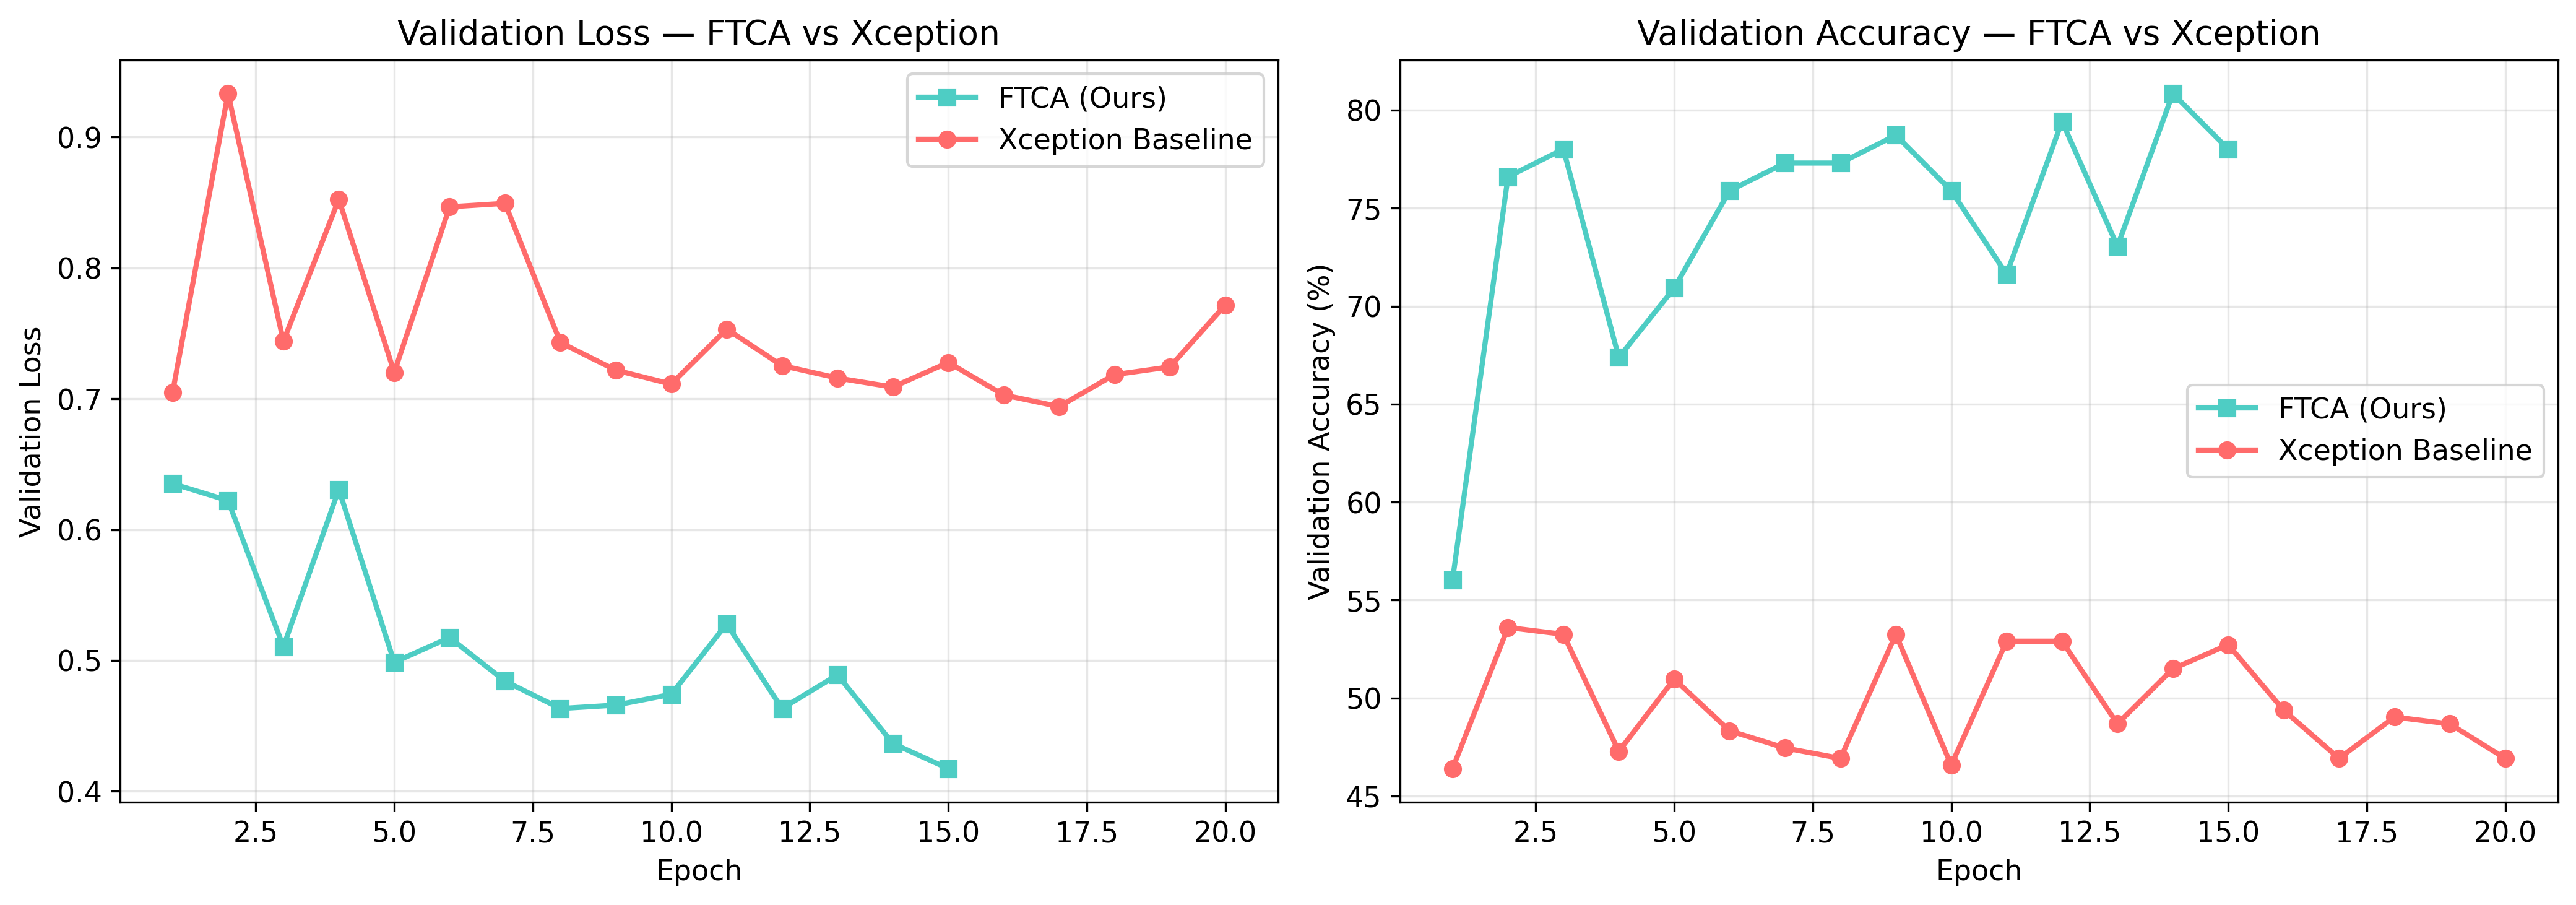
\includegraphics[width=\linewidth]{fig2_ftca_vs_xception.png}
  \caption{FTCA vs Xception validation accuracy comparison across training epochs.}
  \label{fig:comparison}
\end{figure}

\subsection{Latency Analysis}

End-to-end latency averaged 5.2\,s for real webcam sessions, 14.1\,s for phone inputs (higher resolution $\rightarrow$ more MTCNN processing), 8.5\,s for replays, and 7.7\,s for deepfakes. The primary bottleneck is the CPU-bound MTCNN face cropper and the mandatory 6-second rPPG biological buffer ($\approx$180 frames at 30\,fps). Planned optimisations --- RetinaFace or YOLOv8-face and TensorRT INT8 quantisation --- are projected to reduce latency below 3\,s.

% ============================================================
\section{Dataset Composition and Domain Shift}
\label{sec:domain}

C23 compression destroys the microscopic PRNU sensor fingerprint, so the 4 FF++ ``Real'' videos likely triggered the Dynamic Fallback at S1. However, C23 compression is light enough that the macro-pixel chrominance shifts of blood flow survive S3 rPPG extraction. Their successful passage through S4 confirms the FTCA model evaluates genuine deepfake artefacts rather than compression-domain shortcuts --- a cross-domain control validating that the system is not fitting the gap between compressed and uncompressed media.

% ============================================================
\section{Limitations and Future Work}
\label{sec:limits}

\begin{enumerate}
  \item \textbf{Sample Size.} End-to-end validation was conducted on $N=21$ videos, establishing proof-of-concept viability. Large-scale benchmarking requires institutional uncompressed biometric datasets (OULU-NPU, UBFC-rPPG, SiW).
  \item \textbf{FTCA Accuracy.} 80.85\% validation accuracy is strong for a minor project but below production thresholds; more training data and longer training schedules are required.
  \item \textbf{Latency.} 5--15\,s per video is acceptable for batch processing but too slow for real-time UX. TensorRT quantisation and faster face detectors are planned.
  \item \textbf{PRNU on Phones.} Modern computational photography pipelines (HDR+, Night Sight, EIS) destroy PRNU signatures. The Dynamic Fallback partially addresses this, but a dedicated mobile PRNU model would be more robust.
  \item \textbf{Adversarial Robustness.} The system has not been evaluated against perturbations specifically designed to fool individual pipeline stages.
\end{enumerate}

% ============================================================
\section{Conclusion}
\label{sec:conc}

AuthKYC demonstrates that single-layer deepfake detection is fundamentally insufficient for securing banking KYC workflows. By fusing four orthogonal detection principles --- hardware physics (PRNU), frequency-domain optics (Moiré), biological signals (rPPG), and learned spatio-temporal features (FTCA) --- the system forces attackers to simultaneously satisfy physical, biological, and digital constraints. The 95.2\% accuracy with zero false positives on a mixed-domain dataset, combined with a $2\times$ improvement over the Xception spatial baseline, validates this multi-modal cascaded approach as a viable foundation for production PAD systems.

% ============================================================
\section{Code and Artifact Availability}
\label{sec:availability}

The complete source code, training scripts, evaluation pipeline, and module implementations are publicly available:

\begin{itemize}
  \item \textbf{Source Code (GitHub):} \url{https://github.com/mv35011/AuthKYC--END-to-END-system-for-bank-kyc-against-AI-attacks}
  \item \textbf{Trained Weights, Plots, and Artifacts (Google Drive):} \url{https://drive.google.com/drive/folders/1ewJDwSbeyMI3JFJkYBhZD_NDlN92H-8w?usp=sharing}
\end{itemize}

The repository contains: \texttt{modules/} (all 4 security stages), \texttt{core\_engine.py} (orchestrator), \texttt{data/} (training scripts), \texttt{finetune/} (domain adaptation), and \texttt{run\_experiment6.py} (ablation study). Pre-trained model weights (\texttt{patent\_ftca\_v2.pth}) and all report figures are available on the Drive link.

% ============================================================
\balance
\begin{thebibliography}{7}

\bibitem{rossler2019}
A. Rössler, D. Cozzolino, L. Verdoliva, C. Riess, J. Thies, and M. Nießner,
``FaceForensics++: Learning to Detect Manipulated Facial Images,''
in \textit{Proc. IEEE ICCV}, 2019, pp. 1--11.

\bibitem{li2020}
Y. Li, X. Yang, P. Sun, H. Qi, and S. Lyu,
``Celeb-DF: A Large-scale Challenging Dataset for DeepFake Forensics,''
in \textit{Proc. IEEE CVPR}, 2020, pp. 3207--3216.

\bibitem{lukas2006}
J. Luk\'a\v{s}, J. Fridrich, and M. Goljan,
``Digital Camera Identification from Sensor Pattern Noise,''
\textit{IEEE Trans. Inf. Forensics Security}, vol.~1, no.~2, pp. 205--214, 2006.

\bibitem{dehaan2013}
G. de Haan and V. Jeanne,
``Robust Pulse Rate From Chrominance-Based rPPG,''
\textit{IEEE Trans. Biomed. Eng.}, vol.~60, no.~10, pp. 2878--2886, 2013.

\bibitem{tran2018}
D. Tran, H. Wang, L. Torresani, J. Ray, Y. LeCun, and M. Paluri,
``A Closer Look at Spatiotemporal Convolutions for Action Recognition,''
in \textit{Proc. IEEE CVPR}, 2018, pp. 6450--6459.

\bibitem{chollet2017}
F. Chollet,
``Xception: Deep Learning with Depthwise Separable Convolutions,''
in \textit{Proc. IEEE CVPR}, 2017, pp. 1251--1258.

\bibitem{zhang2016}
K. Zhang, Z. Zhang, Z. Li, and Y. Qiao,
``Joint Face Detection and Alignment Using Multitask Cascaded Convolutional Networks,''
\textit{IEEE Signal Process. Lett.}, vol.~23, no.~10, pp. 1499--1503, 2016.

\end{thebibliography}

\end{document}